\documentclass{utmreport}
\usepackage{float,needspace,booktabs}
\providecommand{\tightlist}{\setlength{\itemsep}{0pt}\setlength{\parskip}{0pt}}
\providecommand{\passthrough}[1]{#1}
\providecommand{\pandocbounded}[1]{#1}
\newcounter{none}
\selectlanguage{english}
\institution{Technical University of Moldova}
\faculty{Faculty of Computers, Informatics, and Microelectronics}
\department{Department of Software Engineering}
\studyprogramme{Software Engineering Study Programme}
\documenttype{Laboratory work No. 1}
\reporttitle{Creational design patterns in Domi (C\#)}
\student{Lucian-Adrian Gavril}{FAF-241}
\supervisor{Daniel Istrati}{asist. univ.}
\cityyear{Chișinău}{2026}
\begin{document}
\makeutmreporttitlepage
\tableofcontents
\begin{utmabstract}[Abstract]
This laboratory work applies the six creational design patterns to Domi, a service where people form groups to rent a home together. Builder assembles and validates a group step by step. Abstract Factory produces a group and a suggested renter that always match. Prototype copies a group's settings into a new group without its identity or members. Singleton holds the shared catalog defaults, Factory Method lets subclasses choose the group inside a fixed workflow, and Object Pool reuses buffers for group summaries. For each pattern the report explains the problem it solves, where it fits in Domi, the code, why a simpler approach is not enough, and its disadvantages, and connects the patterns to the SOLID principles from Laboratory work No.~0.

\utmkeywords{creational patterns, builder, abstract factory, prototype, singleton, factory method, object pool}
\end{utmabstract}

\begin{utmabbreviations}
\item[DI] dependency injection
\item[GoF] Gang of Four (Gamma, Helm, Johnson, Vlissides)
\item[ID] identifier
\item[JSON] JavaScript Object Notation
\item[SOLID] single responsibility, open/closed, Liskov substitution, interface segregation, dependency inversion
\item[UML] Unified Modeling Language
\end{utmabbreviations}

\utmintroduction
The task is to study the creational design patterns, implement at least three of them in a project of our choice, and be able to explain the remaining ones. The report must state the project theme, the patterns used, short descriptions with code, and a UML diagram.

The deeper goal is to learn when object creation itself becomes a design problem. Writing \passthrough{\lstinline!new!} is the simplest way to create an object, and for most objects it is enough. The creational patterns answer the cases where it is not enough: when the caller should not know the concrete class, when construction is complicated, when objects must match each other, when a copy is easier than a construction, when only one instance may exist, or when creating an object is too expensive to repeat.

The project is \textbf{Domi}, a service that helps people who do not know each other form a group to rent a home together. Domi is a good fit because creating its objects has real rules: a group must have a valid cost and capacity, a suggested renter must be able to afford the group, and a copied group must not inherit the original\textquotesingle s identity or members.

Implemented in the main demo: \textbf{Builder}, \textbf{Abstract Factory}, \textbf{Prototype}. Implemented as additional examples: \textbf{Singleton}, \textbf{Factory Method}, \textbf{Object Pool}.

\begin{figure}[H]
\centering
\pandocbounded{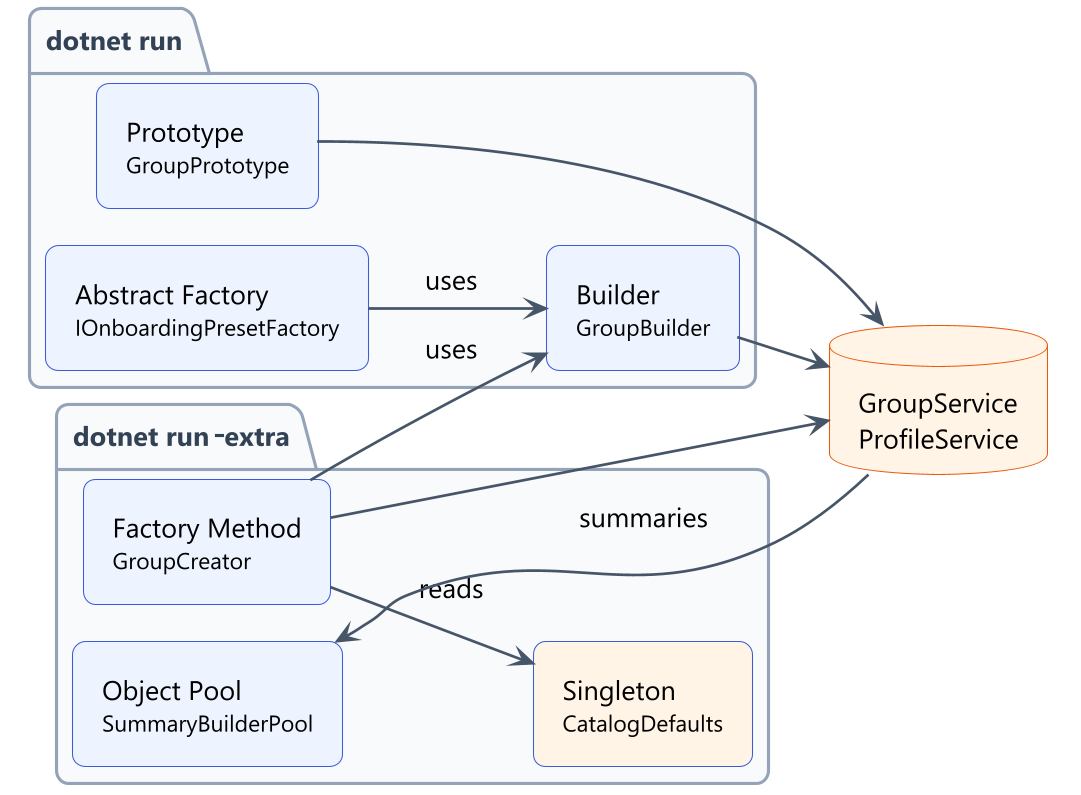
\includegraphics[width=0.92\textwidth,height=0.42\textheight,keepaspectratio]{assets/d01-overview.png}}
\caption*{Figure 1 -- The six patterns in the project and how they relate. Arrows show which pattern uses another.}
\end{figure}

\chapter{Theory: why creational patterns exist}

\section{\texorpdfstring{The problem with \texttt{new} everywhere}{The problem with new everywhere}}

Consider a service that creates groups directly:

\begin{lstlisting}
public GroupView CreateBudgetGroup()
{
    var group = new Group("group-7", new GroupInput("Budget home", 450, 4));
    ...
}
\end{lstlisting}

This works, but three things are now fixed inside the service: the concrete class, the values, and the validation order. When Domi adds a student group, the service must be edited. That is a violation of the \textbf{Open/Closed Principle} from Lab 0 (a module should be open for extension and closed for modification). The service also depends on a concrete class instead of an abstraction, which breaks \textbf{Dependency Inversion}. If several services repeat the same construction steps, the rules drift apart, which breaks \textbf{Single Responsibility}.

Creational patterns fix this by moving the act of creation into one place that the rest of the code calls through an abstraction or a controlled entry point. The code that \emph{uses} an object stops deciding \emph{how} it is made.

\section{The six patterns and the question each one answers}

{\def\LTcaptype{none} % do not increment counter
\begin{longtable}[]{@{}>{\raggedright\arraybackslash}p{0.320\linewidth}>{\raggedright\arraybackslash}p{0.320\linewidth}>{\raggedright\arraybackslash}p{0.320\linewidth}@{}}
\toprule\noalign{}
Pattern & The creation problem it solves & One-line idea \\
\midrule\noalign{}
\endhead
\bottomrule\noalign{}
\endlastfoot
Singleton & Something must exist exactly once & Private constructor, one static instance \\
Factory Method & Same workflow, different object at one step & Subclass overrides the method that creates \\
Abstract Factory & Objects must come in matching families & One factory object creates every member of a family \\
Builder & Construction has many steps or settings that must be valid together & Set values step by step, validate in \passthrough{\lstinline!Build()!} \\
Prototype & A new object should start as a copy of an existing one & The object knows how to clone itself correctly \\
Object Pool & Creating the object is expensive or limited & Reuse released objects instead of creating new ones \\
\end{longtable}
}

The first five come from \emph{Design Patterns: Elements of Reusable Object-Oriented Software} (Gamma, Helm, Johnson, Vlissides, 1994)~\cite{gof}. Object Pool is not in that book but is commonly taught with them because it also controls how instances come into existence.

\section{Class-level and object-level patterns}

The patterns differ in the OOP mechanism they rely on, and this is the clearest way to tell Factory Method from Abstract Factory:

\begin{figure}[H]
\centering
\pandocbounded{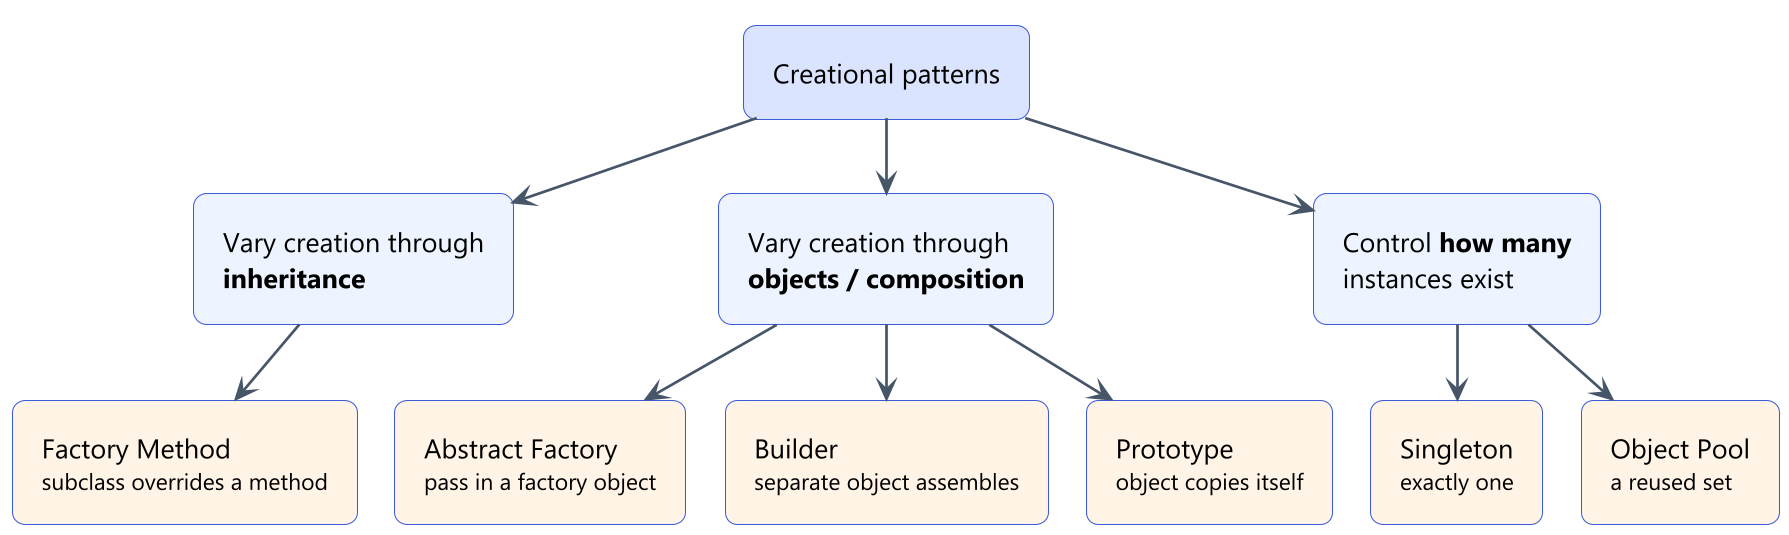
\includegraphics[width=0.92\textwidth,height=0.42\textheight,keepaspectratio]{assets/d02-taxonomy.png}}
\caption{Factory Method varies the created object through inheritance. Abstract Factory, Builder and Prototype vary it through objects. Singleton and Object Pool control the number of instances.}
\end{figure}

\section{OOP terms used in this report}

\begin{itemize}
\tightlist
\item \textbf{Class / object.} \passthrough{\lstinline!Group!} is a class (a blueprint). \passthrough{\lstinline!group-2!} is an object (one concrete group in memory);
\item \textbf{Interface.} A contract of methods without implementation. \passthrough{\lstinline!IOnboardingPresetFactory!} says "you can create a group draft and a profile," without saying how;
\item \textbf{Inheritance.} A child class gets all the parent\textquotesingle s methods and can add or change some. \passthrough{\lstinline!StudentGroupCreator : GroupCreator!};
\item \textbf{Abstract class and method.} \passthrough{\lstinline!GroupCreator!} is abstract: it cannot be created with \passthrough{\lstinline!new!} and exists only to be inherited from. Its \passthrough{\lstinline!abstract!} method has no body, and every child must \passthrough{\lstinline!override!} it;
\item \textbf{Reference.} A variable of class type holds an address, not the object. \passthrough{\lstinline!Group a = b;!} gives two names for one group. This matters for Prototype;
\item \textbf{\passthrough{\lstinline!static!}.} Belongs to the class, not to an object, so there is one copy for the whole program. 100 groups have 100 names but one static field. It does not mean "cannot change". \passthrough{\lstinline!CatalogDefaults.Instance!} is static. This matters for Singleton;
\item \textbf{\passthrough{\lstinline!private!}.} Only code inside the same class can see or change it. \passthrough{\lstinline!\_memberProfileIds!} is private so outside code must go through \passthrough{\lstinline!AddMember!}, which checks the rules;
\item \textbf{\passthrough{\lstinline!override!}.} A child class writes its own version of a method the parent declared \passthrough{\lstinline!abstract!} or \passthrough{\lstinline!virtual!}. When the parent calls that method, the child\textquotesingle s version runs. This is \textbf{polymorphism}. This matters for Factory Method;
\item \textbf{\passthrough{\lstinline!record!}.} A C\# class meant to hold data, with value equality and \passthrough{\lstinline!with!} for making a changed copy. \passthrough{\lstinline!GroupInput!} and \passthrough{\lstinline!ProfileInput!} are records;
\end{itemize}

\chapter{The Domi domain}

Domi has two core objects. A \textbf{Group} has a name, a maximum monthly cost per person, a capacity from 1 to 20, and a list of member IDs. A \textbf{Profile} has a name and a private monthly budget. A profile can join a group only when its budget covers the cost and the group has a free place.

\begin{figure}[H]
\centering
\pandocbounded{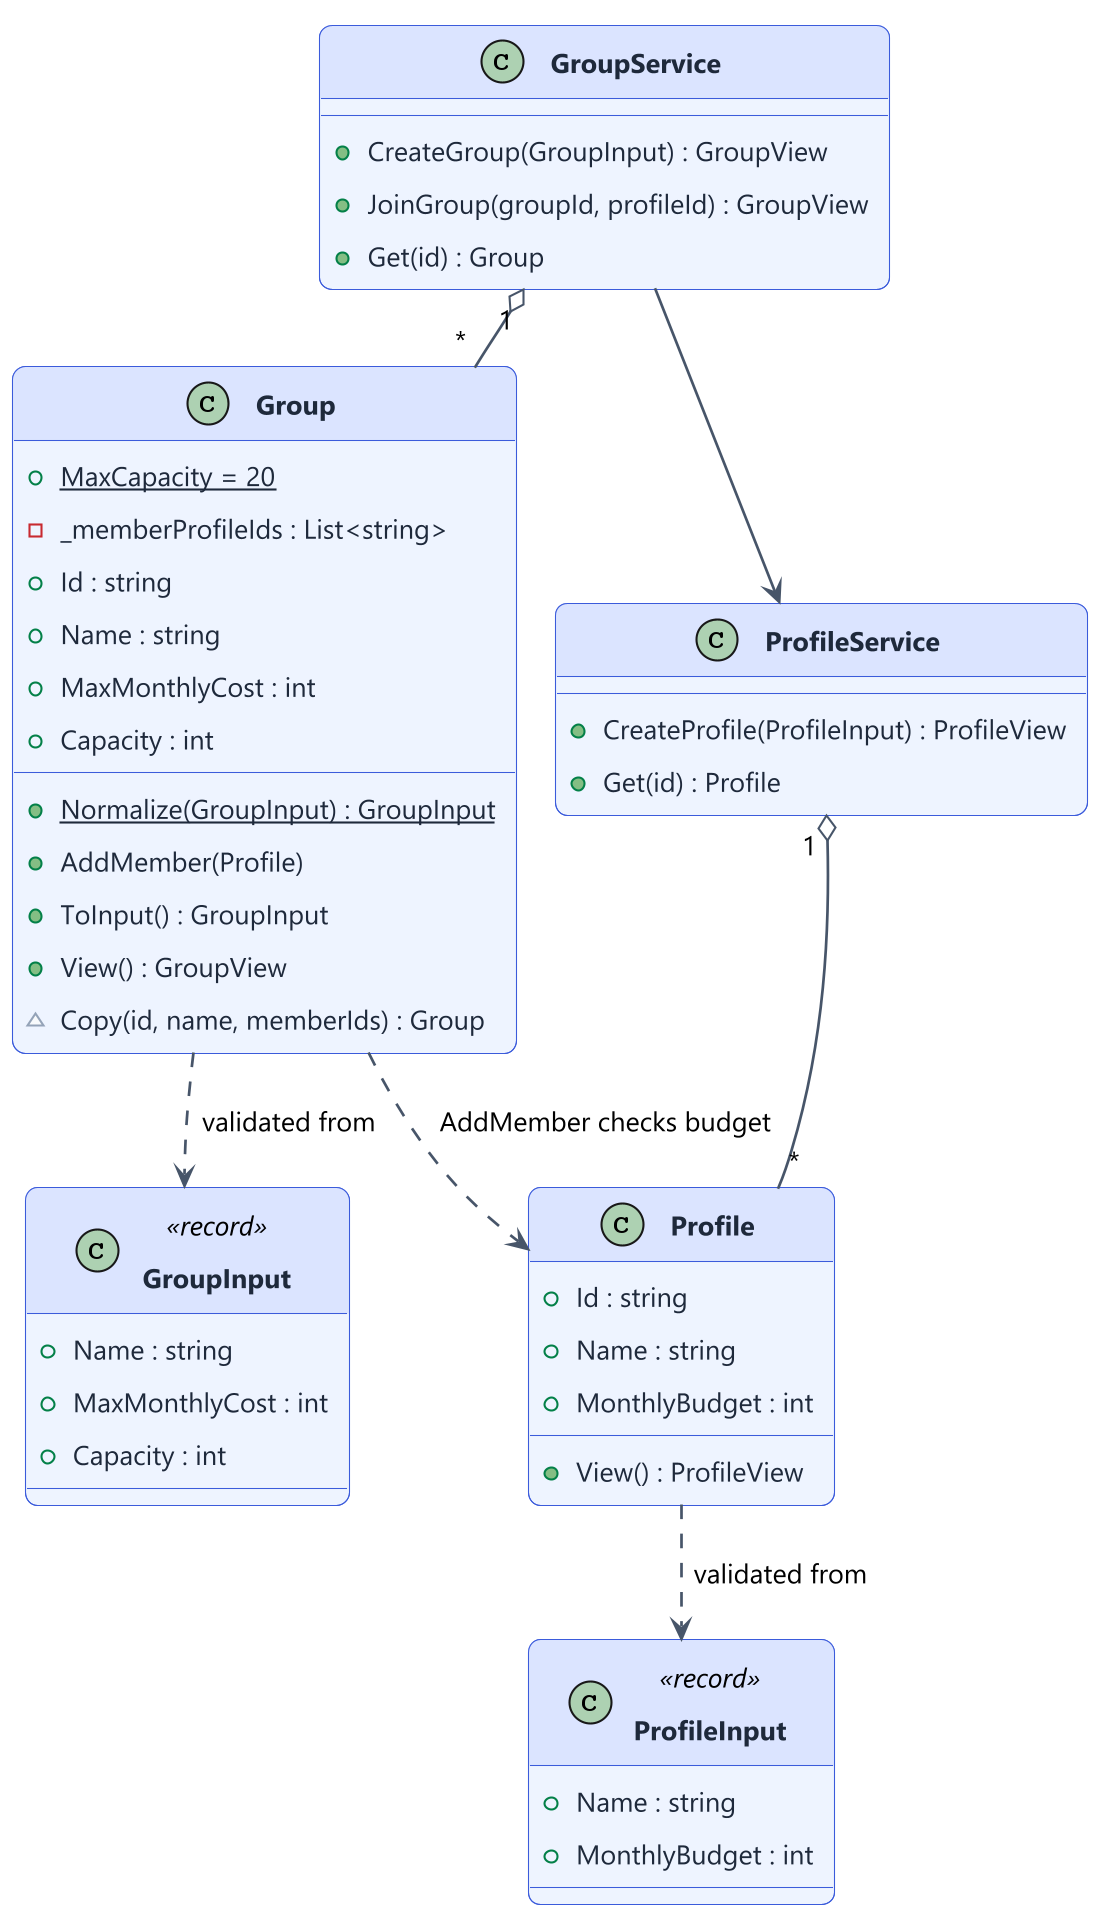
\includegraphics[width=0.92\textwidth,height=0.42\textheight,keepaspectratio]{assets/d03-domain.png}}
\caption{Domain model. Inputs are what a caller sends; the services turn them into stored objects with IDs.}
\end{figure}

\section{One place for the rules}

Every pattern in this lab eventually produces a \passthrough{\lstinline!GroupInput!}, and every \passthrough{\lstinline!GroupInput!} passes through one method:

\begin{lstlisting}
public static GroupInput Normalize(GroupInput input)
{
    string name = (input.Name ?? "").Trim();
    if (name == "") throw new DomainException("group name is required");
    if (input.MaxMonthlyCost <= 0) throw new DomainException("maxMonthlyCost must be greater than zero");
    if (input.Capacity <= 0) throw new DomainException("capacity must be greater than zero");
    if (input.Capacity > MaxCapacity) throw new DomainException($"capacity cannot exceed {MaxCapacity} people");
    return input with { Name = name };
}
\end{lstlisting}

\textbf{How it works.} It trims the name, rejects an empty name, a non-positive cost and a capacity outside 1 to 20, and returns a cleaned copy using \passthrough{\lstinline!with!}. On a rule violation it throws \passthrough{\lstinline!DomainException!}.

\textbf{Why it matters for this lab.} The Builder calls it in \passthrough{\lstinline!Build()!}, the \passthrough{\lstinline!Group!} constructor calls it, and the Prototype calls it through that constructor. Because creation is centralised, no pattern can produce a group the rest of the system would reject.

\section{Joining a group}

\begin{lstlisting}
public void AddMember(Profile profile)
{
    if (_memberProfileIds.Contains(profile.Id)) return;
    if (profile.MonthlyBudget < MaxMonthlyCost) throw new DomainException("monthly budget is below the group's cost");
    if (_memberProfileIds.Count >= Capacity) throw new DomainException("group is full");
    _memberProfileIds.Add(profile.Id);
}
\end{lstlisting}

\textbf{How it works.} A repeated join returns without error, so retrying a request is safe. Then it checks the budget and the capacity \emph{before} changing anything, so a failed join leaves the group unchanged. Only after both checks does it add the ID.

\begin{figure}[H]
\centering
\pandocbounded{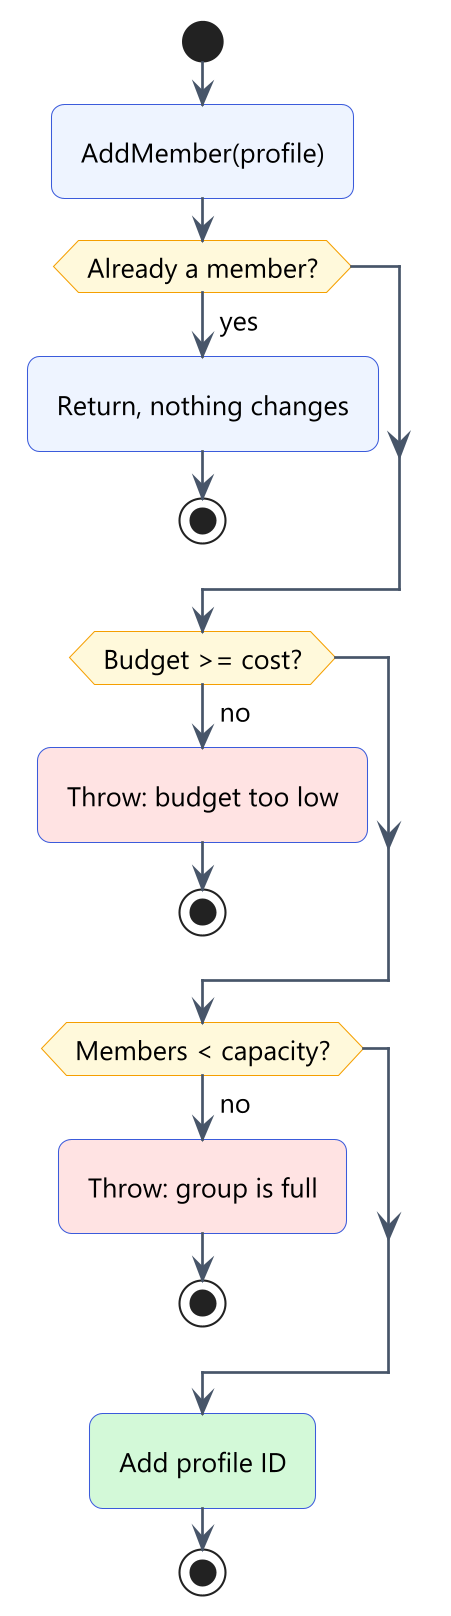
\includegraphics[width=0.92\textwidth,height=0.42\textheight,keepaspectratio]{assets/d04-join.png}}
\caption{The join rule. Every check happens before the member list changes.}
\end{figure}

\chapter{Builder}

\section{The idea in plain words}

Think of ordering at a sandwich shop. You don\textquotesingle t shout everything in one breath. You say "white bread", then "chicken", then "no onions", then "that\textquotesingle s it, make it". The worker collects your choices one by one and only makes the sandwich at the end. If you forgot to choose bread, they stop you at the end, before making anything.

A Builder works the same way. You give it values one at a time with methods that say what each value is (\passthrough{\lstinline!WithName!}, \passthrough{\lstinline!WithCapacity!}), and at the end you call \passthrough{\lstinline!Build()!}. Only then does it check everything and make the object.

\section{Problem it solves}

\textbf{Problem 1: mixed-up values.} A group needs a name, a cost and a capacity. With a normal constructor you pass them in order:

\begin{lstlisting}
new GroupInput("Flat", 450, 4);   // name, cost, capacity
\end{lstlisting}

Cost and capacity are both \passthrough{\lstinline!int!}. If someone swaps them, \passthrough{\lstinline!new GroupInput("Flat", 4, 6)!}, it still compiles and passes validation, because 4 and 6 are both allowed values. Domi now has a group that costs 4 per month for 6 people, and nobody gets an error. With a Builder the call says \passthrough{\lstinline!.WithMaxMonthlyCost(450).WithCapacity(4)!}, so a swap is visible when you read it.

\textbf{Problem 2: too many constructors.} Domi will grow: city, pets allowed, smoking, move-in date. Some groups set them and some don\textquotesingle t. With constructors you end up writing one for every combination:

\begin{lstlisting}
new GroupInput(name, cost, capacity)
new GroupInput(name, cost, capacity, city)
new GroupInput(name, cost, capacity, city, pets)
new GroupInput(name, cost, capacity, city, pets, smoking, moveIn)
\end{lstlisting}

This growing list is called the \textbf{telescoping constructor} problem. With a Builder you call only the \passthrough{\lstinline!With...!} methods you need, and the rest keep their defaults.

\textbf{Problem 3: checking values together.} Some rules involve several values at once. Checking them in the middle, after only the name is set, would fail because the cost isn\textquotesingle t set yet. The Builder waits until \passthrough{\lstinline!Build()!}, when everything is there, and checks it all at once.

\section{Where it fits in Domi}

The "create group" form collects fields one at a time, and the user presses \emph{Create} at the end. The Builder has the same shape: set values in any order, validate once at the end. Other real uses: \passthrough{\lstinline!StringBuilder!} in C\# (append text piece by piece, then \passthrough{\lstinline!ToString()!}), building an SQL query or an HTTP request with optional parts, and \passthrough{\lstinline!WebApplication.CreateBuilder()!} in ASP.NET.

\section{Code}

\begin{lstlisting}
public sealed class GroupBuilder
{
    private string _name = "";
    private int _maxMonthlyCost;
    private int _capacity;

    public GroupBuilder WithName(string name)
    {
        _name = name;
        return this;
    }

    public GroupBuilder WithMaxMonthlyCost(int amount)
    {
        _maxMonthlyCost = amount;
        return this;
    }

    public GroupBuilder WithCapacity(int people)
    {
        _capacity = people;
        return this;
    }

    public GroupInput Build() => Group.Normalize(new GroupInput(_name, _maxMonthlyCost, _capacity));
}
\end{lstlisting}

Usage in \passthrough{\lstinline!Program.cs!}:

\begin{lstlisting}
GroupInput builderInput = new GroupBuilder()
    .WithName("Builder example home")
    .WithMaxMonthlyCost(650)
    .WithCapacity(3)
    .Build();
GroupView builderGroup = groups.CreateGroup(builderInput);
\end{lstlisting}

\section{How it works}

Each \passthrough{\lstinline!With...!} method stores one value in a private field and returns \passthrough{\lstinline!this!}, the same builder object. Because the return type is \passthrough{\lstinline!GroupBuilder!}, the next call can be chained directly, which is called a \textbf{fluent interface}. No validation runs while values are being set, so the order of calls does not matter and an incomplete builder is never mistaken for a finished group. \passthrough{\lstinline!Build()!} creates the record and passes it to \passthrough{\lstinline!Group.Normalize!}, which validates all three values together and either returns a clean input or throws.

The Builder returns a \passthrough{\lstinline!GroupInput!}, not a saved \passthrough{\lstinline!Group!}. Saving and assigning an ID is the service\textquotesingle s job. The Builder only knows how to assemble a valid request, which keeps its responsibility small.

\begin{figure}[H]
\centering
\pandocbounded{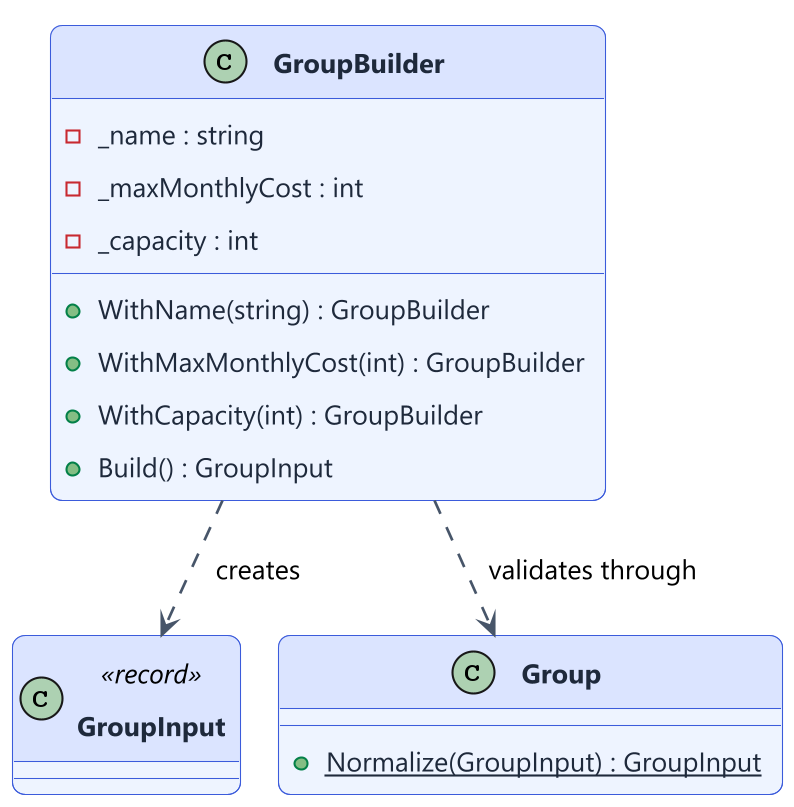
\includegraphics[width=0.92\textwidth,height=0.42\textheight,keepaspectratio]{assets/d05-builder-class.png}}
\caption{Builder class diagram.}
\end{figure}

\begin{figure}[H]
\centering
\pandocbounded{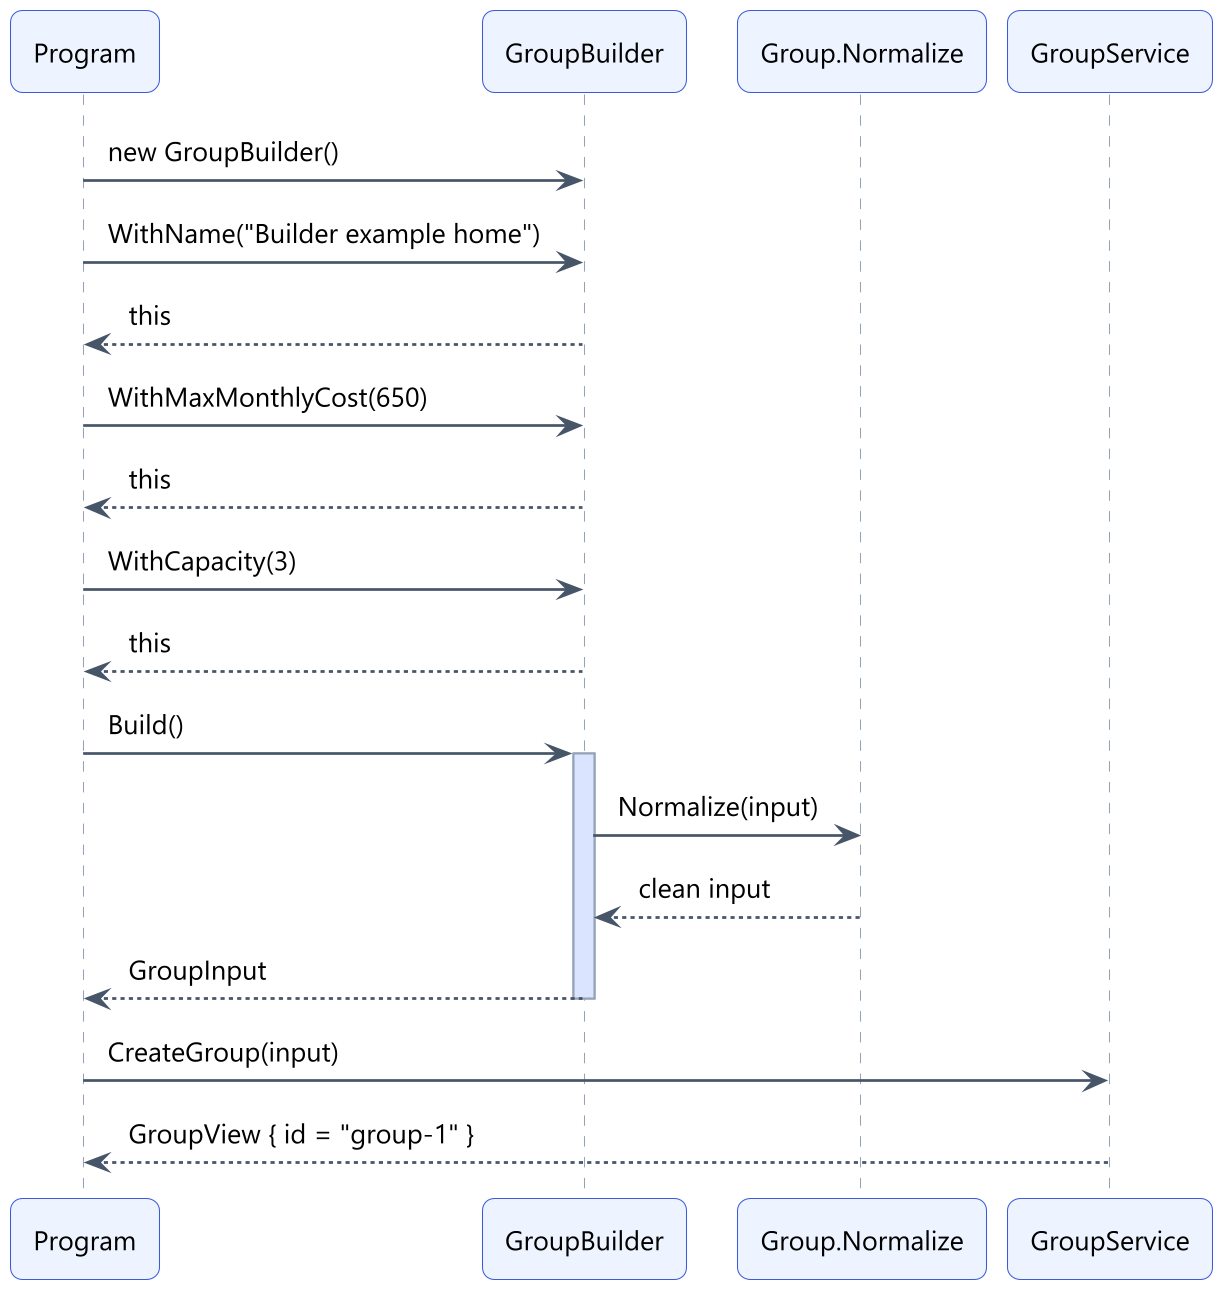
\includegraphics[width=0.92\textwidth,height=0.42\textheight,keepaspectratio]{assets/d06-builder-seq.png}}
\caption{Builder sequence. Validation happens once, in \protect\passthrough{\lstinline!Build()!}.}
\end{figure}

\section{Why not something simpler}

C\# named arguments, \passthrough{\lstinline!new GroupInput(Name: "Flat", MaxMonthlyCost: 450, Capacity: 4)!}, already fix the mixed-up values problem. A Builder is worth its extra class when values arrive in separate steps (a multi-page form, defaults that some callers override) or when validation must see all values together. Domi\textquotesingle s onboarding factories use the Builder with partly fixed values, which is the second case.

\section{Disadvantages}

A pattern always costs something. For the Builder:

\begin{enumerate}
\def\labelenumi{\arabic{enumi}.}
\tightlist
\item \textbf{More code.} For every class you build, you write a second class (\passthrough{\lstinline!GroupBuilder!}) with a field and a method for each value. Add a field to \passthrough{\lstinline!Group!} and you must remember to add it to the Builder too;
\item \textbf{Overkill for small objects.} For an object with two values, \passthrough{\lstinline!new Point(3, 5)!} is clearer than \passthrough{\lstinline!new PointBuilder().WithX(3).WithY(5).Build()!}. The Builder only pays off when there are many values or optional ones;
\item \textbf{Errors appear later.} A wrong value is reported at \passthrough{\lstinline!Build()!}, not on the line where you set it, so the error points to the end of the chain, not to the mistake;
\item \textbf{Forgotten values are not caught by the compiler.} If you forget \passthrough{\lstinline!.WithCapacity(...)!}, the code still compiles, and the problem only shows up when the program runs and \passthrough{\lstinline!Build()!} throws. A constructor with a required parameter would refuse to compile;
\item \textbf{Reusing a builder keeps old values.} Call \passthrough{\lstinline!Build()!} twice on the same builder and the second object starts with the first one\textquotesingle s values. Start each object with \passthrough{\lstinline!new GroupBuilder()!};
\end{enumerate}

\textbf{When to use it:} many values, optional values, or rules that check values together. \textbf{When not to:} two or three required values, where a constructor or named arguments are enough.

\chapter{Abstract Factory}

\section{The idea in plain words}

Think of furniture styles in a store. If you pick the "Modern" style, you get a modern chair \emph{and} a modern table. You never get a modern chair with a vintage table, because one choice of style gives you the whole matching set.

An Abstract Factory is that style. It is an \textbf{interface} listing everything in the set ("create a group", "create a renter"), and each class that implements it creates one matching family. The code that uses it receives one factory and asks it for every part, so the parts always match.

\section{Problem}

Domi\textquotesingle s onboarding suggests a group and a renter profile together. They only make sense as a pair: a budget renter with 500 per month cannot join a comfort group at 700. If the code chooses the group and the profile in two separate places, nothing prevents a mismatched pair, and the first join fails.

\section{Where it fits in Domi}

The onboarding screen asks once: \emph{Budget} or \emph{Comfort}. That single choice must give a matching group and profile. Each style is a \textbf{family} of related objects.

\section{Code}

\begin{lstlisting}
public sealed record OnboardingPreset(GroupInput Group, ProfileInput SuggestedProfile);

public interface IOnboardingPresetFactory
{
    GroupInput CreateGroupDraft();
    ProfileInput CreateSuggestedProfile();
}

public sealed class BudgetPresetFactory : IOnboardingPresetFactory
{
    public GroupInput CreateGroupDraft() => new GroupBuilder()
        .WithName("Budget shared home")
        .WithMaxMonthlyCost(450)
        .WithCapacity(4)
        .Build();

    public ProfileInput CreateSuggestedProfile() => Presets.ProfileSuggestion("Budget renter", 500);
}

public sealed class ComfortPresetFactory : IOnboardingPresetFactory
{
    public GroupInput CreateGroupDraft() => new GroupBuilder()
        .WithName("Comfort shared home")
        .WithMaxMonthlyCost(700)
        .WithCapacity(2)
        .Build();

    public ProfileInput CreateSuggestedProfile() => Presets.ProfileSuggestion("Comfort renter", 900);
}
\end{lstlisting}

The client code:

\begin{lstlisting}
public static OnboardingPreset Build(IOnboardingPresetFactory factory)
{
    GroupInput group = factory.CreateGroupDraft();
    ProfileInput profile = factory.CreateSuggestedProfile();

    if (profile.MonthlyBudget < group.MaxMonthlyCost)
        throw new DomainException("monthly budget is below the group's cost");

    return new OnboardingPreset(group, profile);
}
\end{lstlisting}

\section{How it works}

The interface declares one creation method per product in the family. Each concrete factory implements all of them for one family, so the Budget factory can only produce budget products. \passthrough{\lstinline!Presets.Build!} receives the factory as an \passthrough{\lstinline!IOnboardingPresetFactory!} and never mentions \passthrough{\lstinline!BudgetPresetFactory!} or \passthrough{\lstinline!ComfortPresetFactory!}. It asks for both products and checks that they fit before returning the pair.

The demo loops over both families, saves each group and profile, and joins them:

\begin{lstlisting}
foreach (var (name, factory) in families)
{
    OnboardingPreset preset = Presets.Build(factory);
    GroupView group = groups.CreateGroup(preset.Group);
    ProfileView profile = profiles.CreateProfile(preset.SuggestedProfile);
    GroupView joined = groups.JoinGroup(group.Id, profile.Id);
    ...
}
\end{lstlisting}

Both joins succeed, which shows that each family is internally consistent.

\begin{figure}[H]
\centering
\pandocbounded{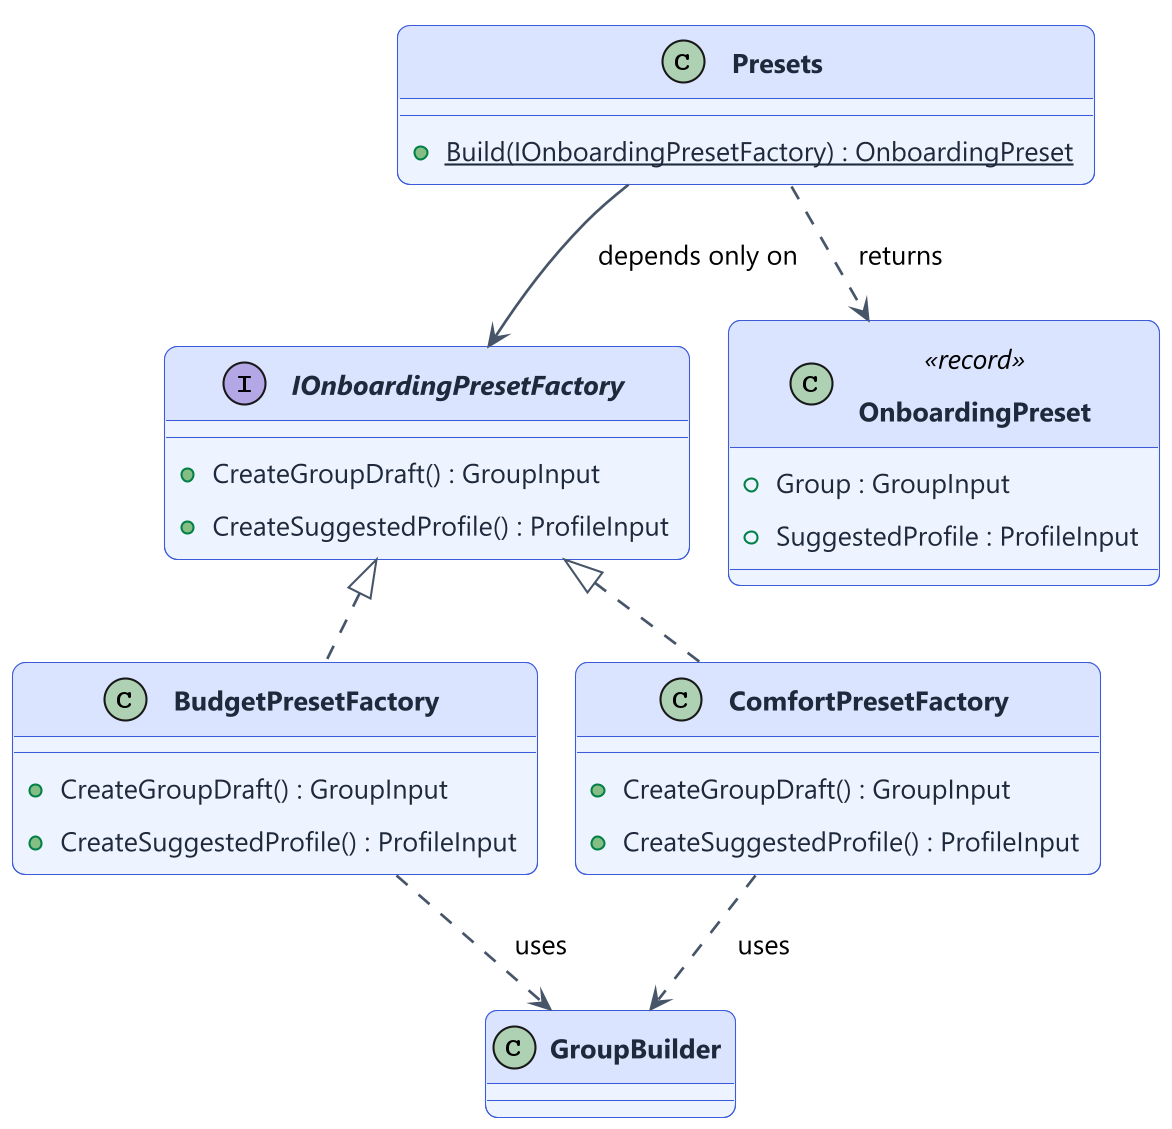
\includegraphics[width=0.92\textwidth,height=0.42\textheight,keepaspectratio]{assets/d07-af-class.png}}
\caption{Abstract Factory class diagram. The client depends on the interface only.}
\end{figure}

\begin{figure}[H]
\centering
\pandocbounded{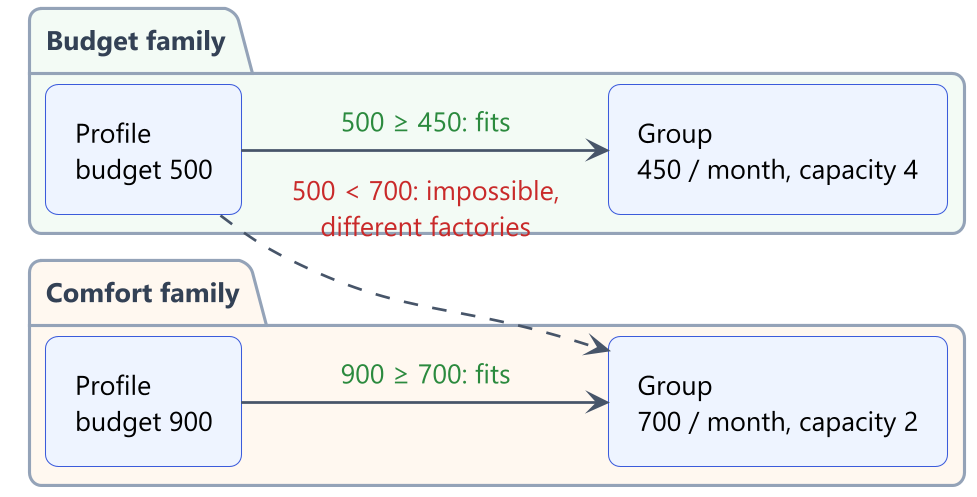
\includegraphics[width=0.92\textwidth,height=0.42\textheight,keepaspectratio]{assets/d08-af-families.png}}
\caption{Each factory produces a matching pair. A cross-family pair cannot be produced because one factory creates both products.}
\end{figure}

\section{Why not something simpler}

The alternative is two \passthrough{\lstinline!switch!} statements, one choosing the group and one choosing the profile. When a third style is added, both must be updated, and forgetting one creates exactly the mismatch above. With the factory, a new \emph{Student} family is one new class, and \passthrough{\lstinline!Presets.Build!} and the demo loop do not change. That is the Open/Closed Principle in practice, and the client depending on the interface instead of concrete classes is Dependency Inversion.

\section{Trade-offs}

Adding a new \textbf{family} is cheap: one class. Adding a new \textbf{product} to every family (for example, a suggested apartment) is expensive: the interface and every factory must change. Abstract Factory is a good choice when families change more often than the kinds of products in them.

\begin{figure}[H]
\centering
\pandocbounded{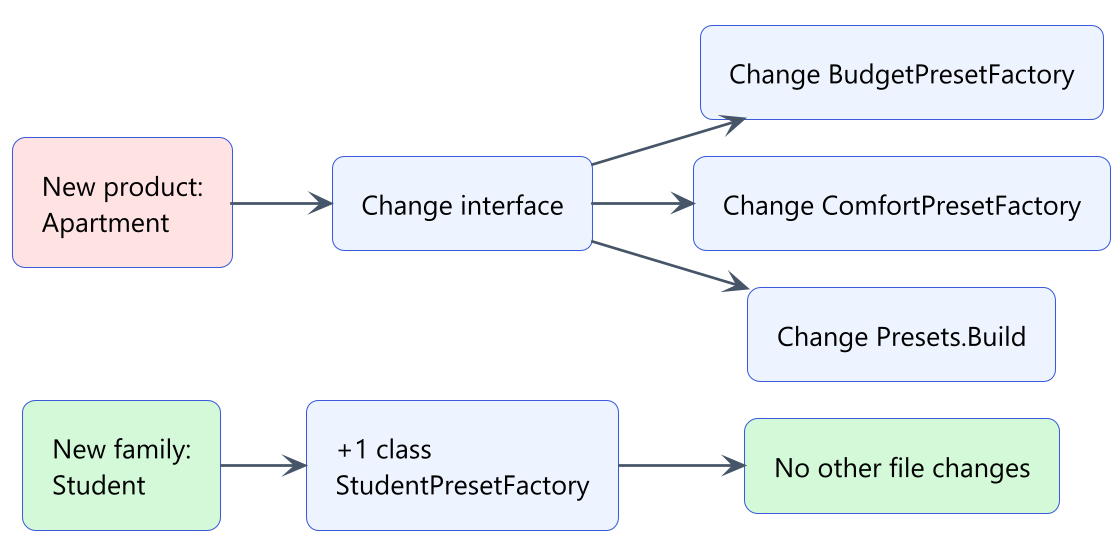
\includegraphics[width=0.92\textwidth,height=0.42\textheight,keepaspectratio]{assets/d09-af-tradeoff.png}}
\caption{The Abstract Factory trade-off: families are cheap to add, product types are not.}
\end{figure}

\chapter{Prototype}

\section{The idea in plain words}

Think of a form you already filled in last year. Instead of filling a blank one again, you photocopy it, then cross out your old signature and date. You keep what is still useful and remove what belonged only to the original.

A Prototype creates a new object by \textbf{copying an existing one}, then resetting what must be unique. In Domi: copy a group\textquotesingle s cost and capacity, give it a new name, and leave out the ID and the members.

To copy correctly you need to know what a \textbf{reference} is. A variable of a class type does not hold the object; it holds the object\textquotesingle s address in memory.

\begin{lstlisting}
Group a = new Group(...);  // one object in memory, a holds its address
Group b = a;               // b gets the same address: still ONE object
b.AddMember(x);            // a sees x too, because it is the same object
\end{lstlisting}

So \passthrough{\lstinline!Group b = a;!} is not a copy. A real copy needs a new object, and inside it, new copies of any lists.

\section{Problem}

A user wants "a group like this one": the same cost and capacity, a new name, and nobody in it yet. Copying the fields from outside forces the caller to know every field, and it breaks when a field is added. Assigning the object (\passthrough{\lstinline!Group copy = source;!}) creates no copy at all, just a second reference to the same group.

\section{Where it fits in Domi}

A \emph{Duplicate group} action, or reusing last semester\textquotesingle s group settings for a new group.

\section{Code}

\begin{lstlisting}
public sealed class GroupPrototype
{
    private readonly Group _template;

    public GroupPrototype(Group source)
    {
        _template = source.Copy(source.Id, source.Name, source.MemberProfileIds);
    }

    public Group CloneAsDraft(string name) => _template.Copy(id: "", name: name, memberIds: []);
}
\end{lstlisting}

The copy itself lives inside \passthrough{\lstinline!Group!}, because only \passthrough{\lstinline!Group!} can reach its private member list:

\begin{lstlisting}
internal Group Copy(string id, string name, IEnumerable<string> memberIds)
{
    Group copy = new(id, new GroupInput(name, MaxMonthlyCost, Capacity));
    copy._memberProfileIds.AddRange(memberIds);
    return copy;
}
\end{lstlisting}

Usage:

\begin{lstlisting}
Group source = groups.Get(budgetGroupId);
GroupPrototype prototype = new(source);
Group draft = prototype.CloneAsDraft("Budget shared home copy");
GroupView copy = groups.CreateGroup(draft.ToInput());
\end{lstlisting}

\section{How it works}

The constructor takes a \textbf{snapshot} of the source. \passthrough{\lstinline!Copy!} creates a brand-new \passthrough{\lstinline!Group!} through the normal constructor (so validation runs) and fills a \textbf{new} list with the source\textquotesingle s member IDs. Later changes to the source cannot affect the snapshot.

\passthrough{\lstinline!CloneAsDraft!} copies the snapshot again, keeping cost and capacity, but with an empty ID, a new name and no members. The service then saves the draft and assigns a fresh ID.

Two things are deliberately not copied:

\begin{itemize}
\tightlist
\item \textbf{The ID.} It is the identity of the original record. Two records with the same ID would be the same group to the store, which is a bug;
\item \textbf{The members.} They joined the original group. A new group starts empty;
\end{itemize}

\section{Shallow copy and deep copy}

This is the central idea of Prototype. A field of type \passthrough{\lstinline!List<string>!} does not hold the list; it holds a \textbf{reference} to it. A \textbf{shallow copy} copies field values, so the copy receives the same reference, and both groups point to one list. A \textbf{deep copy} creates a new list.

\begin{figure}[H]
\centering
\pandocbounded{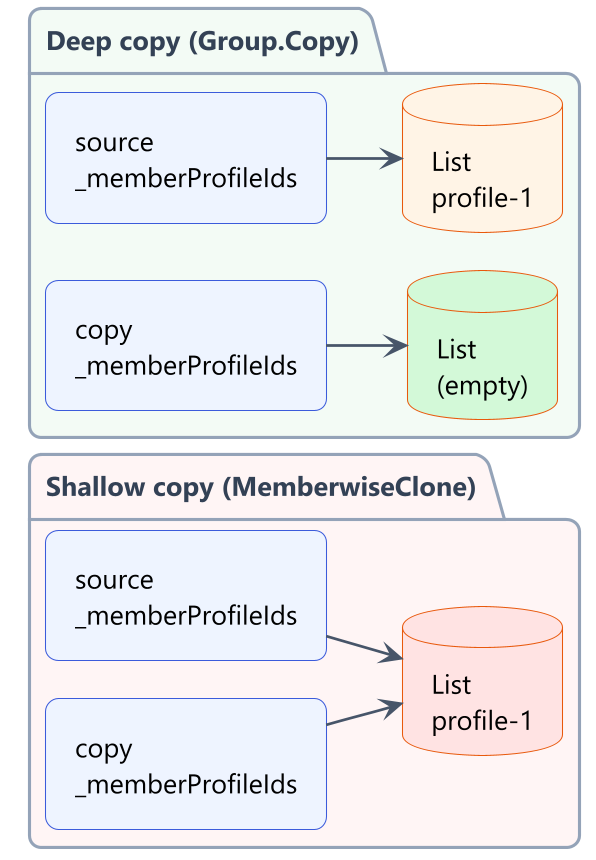
\includegraphics[width=0.92\textwidth,height=0.42\textheight,keepaspectratio]{assets/d10-shallow-deep.png}}
\caption{With a shallow copy, adding a member to the copy also adds it to the source, because there is only one list. The deep copy gives each group its own list.}
\end{figure}

C\# offers \passthrough{\lstinline!object.MemberwiseClone()!}, which performs a shallow copy, and the \passthrough{\lstinline!ICloneable!} interface, which does not say whether its \passthrough{\lstinline!Clone()!} is shallow or deep. Both are reasons this lab writes the copy explicitly.

\begin{figure}[H]
\centering
\pandocbounded{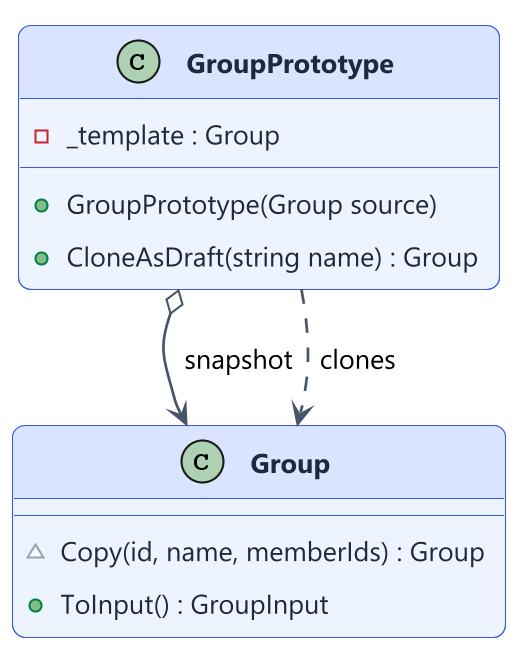
\includegraphics[width=0.92\textwidth,height=0.42\textheight,keepaspectratio]{assets/d11-prototype-class.png}}
\caption{Prototype class diagram.}
\end{figure}

\begin{figure}[H]
\centering
\pandocbounded{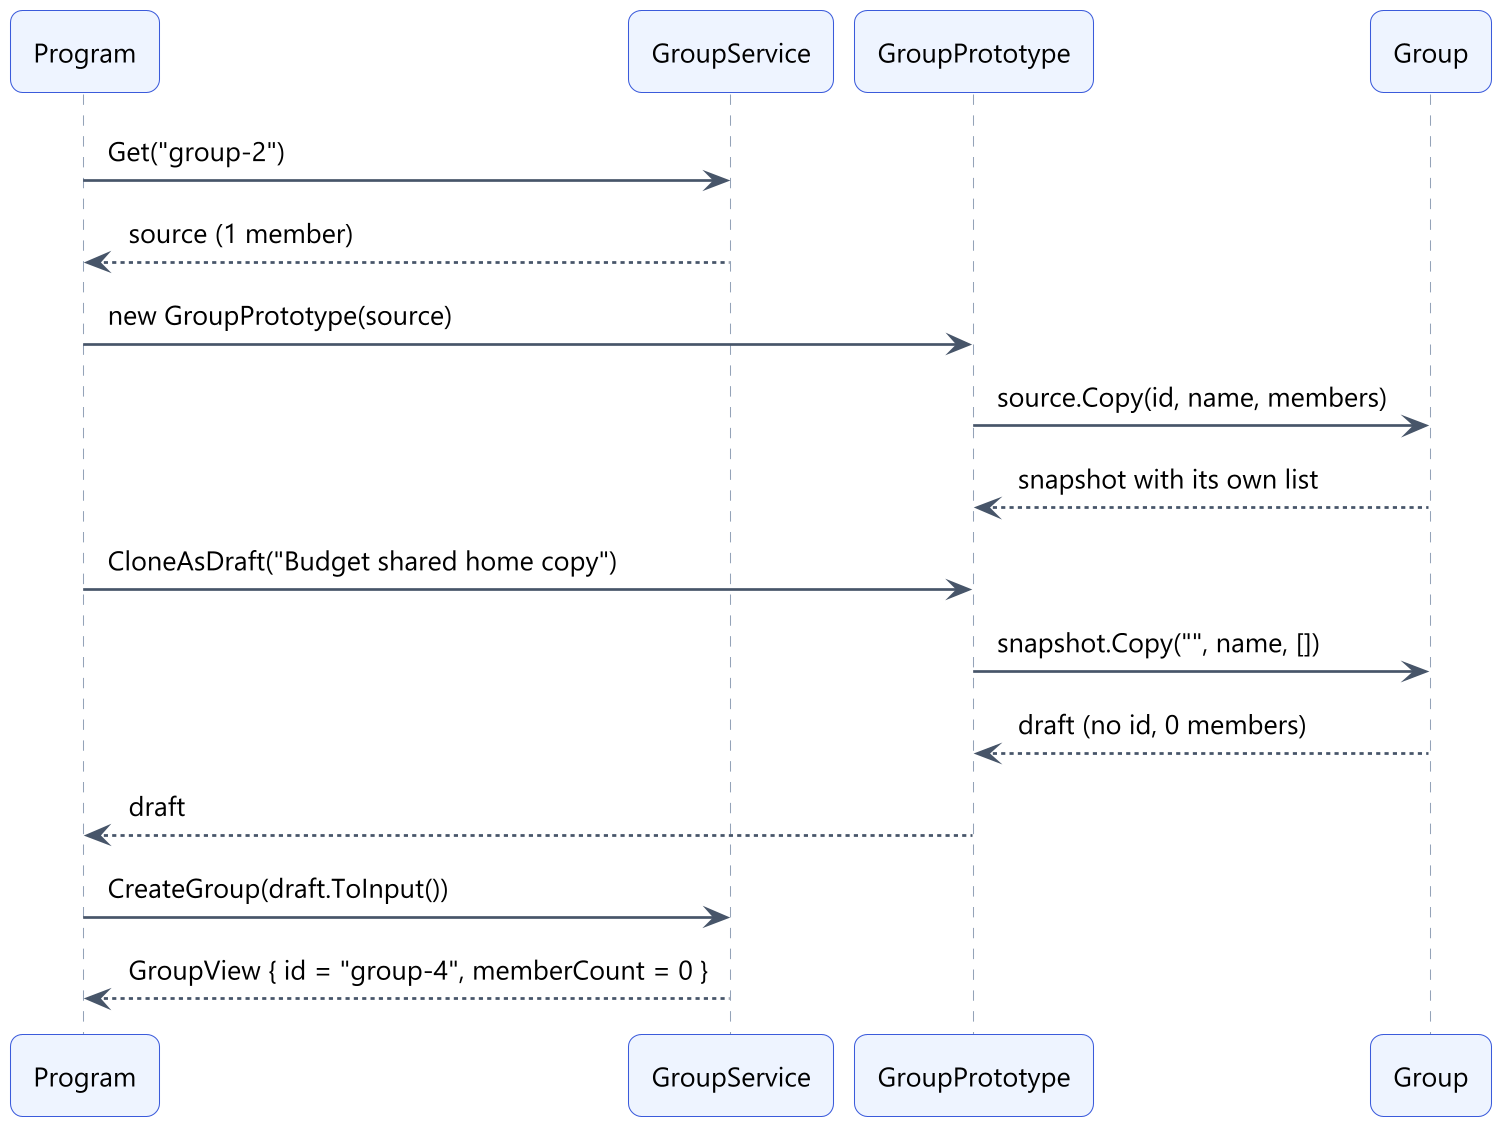
\includegraphics[width=0.92\textwidth,height=0.42\textheight,keepaspectratio]{assets/d12-prototype-seq.png}}
\caption{Prototype sequence. The copy receives a new ID from the service.}
\end{figure}

\section{Trade-offs}

Every new field forces a decision: copy it, deep-copy it, or reset it. A forgotten field produces a wrong copy without any error. Objects with references to other objects (graphs, cycles) make deep copying harder.

\chapter{Singleton}

\section{\texorpdfstring{First, what \texttt{static} means}{First, what static means}}

A normal field belongs to \textbf{each object}. A \passthrough{\lstinline!static!} field belongs to the \textbf{class itself}, so there is exactly one of it in the whole program.

Think of a classroom. Every student has their own notebook (a normal field), and there is one whiteboard on the wall that everyone shares (a static field).

\begin{lstlisting}
class Student
{
    public string Name;            // notebook: each student has their own
    public static string Board;    // whiteboard: one for all students
}
\end{lstlisting}

With 100 \passthrough{\lstinline!Student!} objects there are 100 \passthrough{\lstinline!Name!} values but still only one \passthrough{\lstinline!Board!}, read through the class name: \passthrough{\lstinline!Student.Board!}.

Static does \textbf{not} mean "cannot change". That is \passthrough{\lstinline!const!} or \passthrough{\lstinline!readonly!}. Static means "one shared copy".

\section{The idea in plain words}

A Singleton is a class that allows \textbf{only one object of itself to ever exist}, and gives everyone the same way to reach it.

Think of a school bell. The school has one bell, and every classroom hears the same one. If each classroom had its own bell ringing at a slightly different time, nobody would know when the break starts.

A static field is one shared \emph{variable}. A Singleton uses one static field to hold one shared \emph{object}, and blocks everyone from creating a second one.

\section{Problem it solves}

Some things must exist only once in a program, because two copies would disagree or waste something scarce:

\begin{itemize}
\tightlist
\item \textbf{Configuration.} If two config objects were loaded at different times, one part of the program could use the old database address and another part the new one;
\item \textbf{A logger.} Two loggers writing to the same file at once would mix their lines together;
\item \textbf{A single device.} One printer queue or one connection to a hardware sensor. Two objects controlling it would send conflicting commands;
\end{itemize}

\section{Where it fits in Domi}

Domi\textquotesingle s catalog defaults (default capacity 3, default cost 500) are the same for the whole application. Every part of the program must see the same values. The group creators in section 8 read them through \passthrough{\lstinline!CatalogDefaults.Instance!}.

\section{Where Singleton is used in real software}

{\def\LTcaptype{none} % do not increment counter
\begin{longtable}[]{@{}>{\raggedright\arraybackslash}p{0.480\linewidth}>{\raggedright\arraybackslash}p{0.480\linewidth}@{}}
\toprule\noalign{}
Use & Why one instance \\
\midrule\noalign{}
\endhead
\bottomrule\noalign{}
\endlastfoot
Application configuration & Everyone must read the same settings \\
Logger & All log lines go through one writer, in order \\
Cache & One shared memory of results, so work is not repeated \\
Connection pool & One pool object manages all database connections (section 9) \\
\passthrough{\lstinline!HttpClient!} in .NET & Microsoft recommends sharing one instance; creating many runs out of network sockets \\
\end{longtable}
}

\section{Where Singleton should NOT be used}

\begin{itemize}
\tightlist
\item \textbf{User data: groups, profiles, a shopping cart, the current user.} There are many of them, one per person. A Singleton \passthrough{\lstinline!CurrentUser!} on a server would make every visitor the same user;
\item \textbf{Anything that changes often and is read by many parts of the program.} One shared object that everyone can modify means any part of the code can break any other part, and bugs are hard to trace;
\item \textbf{Things you need to replace in tests.} Code that calls \passthrough{\lstinline!CatalogDefaults.Instance!} directly always gets the real object. A test cannot give it fake values;
\item \textbf{Just to avoid passing a parameter.} "It\textquotesingle s easier to reach from everywhere" is not a reason. That turns it into a global variable;
\end{itemize}

\section{Code}

\begin{lstlisting}
public sealed class CatalogDefaults
{
    private static readonly Lazy<CatalogDefaults> _instance = new(() => new CatalogDefaults());

    public static CatalogDefaults Instance => _instance.Value;

    private CatalogDefaults() { }

    public int DefaultCapacity { get; } = 3;
    public int DefaultMaxMonthlyCost { get; } = 500;
}
\end{lstlisting}

\section{How it works}

Three parts make it a Singleton, and each one answers a question:

\begin{itemize}
\tightlist
\item \textbf{How do we stop people creating a second one?} \passthrough{\lstinline!private CatalogDefaults()!}: no code outside the class can write \passthrough{\lstinline!new CatalogDefaults()!};
\item \textbf{Where is the one object kept?} \passthrough{\lstinline!static ... \_instance!}: the field belongs to the class, so there is one for the whole program (the whiteboard);
\item \textbf{How does everyone reach it?} \passthrough{\lstinline!public static Instance!}: anyone writes \passthrough{\lstinline!CatalogDefaults.Instance!} and gets that same object;
\end{itemize}

Two details make it safe:

\begin{itemize}
\tightlist
\item \passthrough{\lstinline!Lazy<T>!}: creates the object the first time \passthrough{\lstinline!.Value!} is read and guarantees, by default, that this happens once even when several threads ask at the same moment~\cite{lazy};
\item \passthrough{\lstinline!sealed!}: no subclass can add a second constructor path;
\item Properties have only \passthrough{\lstinline!get!}, so the shared object cannot be changed;
\end{itemize}

The demo prints \passthrough{\lstinline!Singleton same instance: True!} by comparing two reads with \passthrough{\lstinline!ReferenceEquals!}.

\begin{figure}[H]
\centering
\pandocbounded{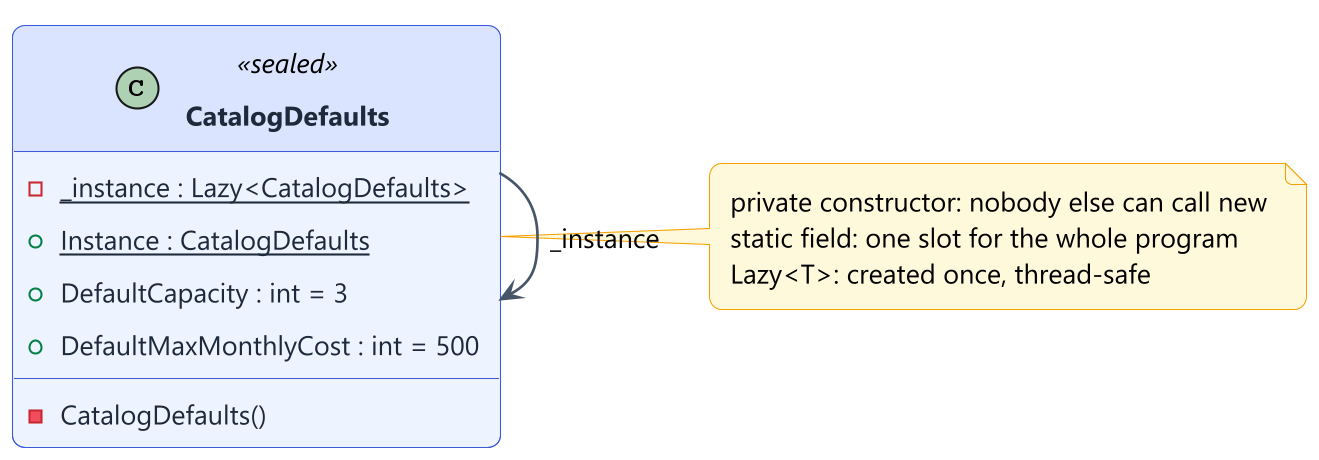
\includegraphics[width=0.92\textwidth,height=0.42\textheight,keepaspectratio]{assets/d13-singleton-class.png}}
\caption{Singleton class diagram. The class holds its only instance.}
\end{figure}

\section{Why thread safety matters}

The naive version checks and creates in two steps:

\begin{lstlisting}
if (_instance == null) _instance = new Config();
return _instance;
\end{lstlisting}

\begin{figure}[H]
\centering
\pandocbounded{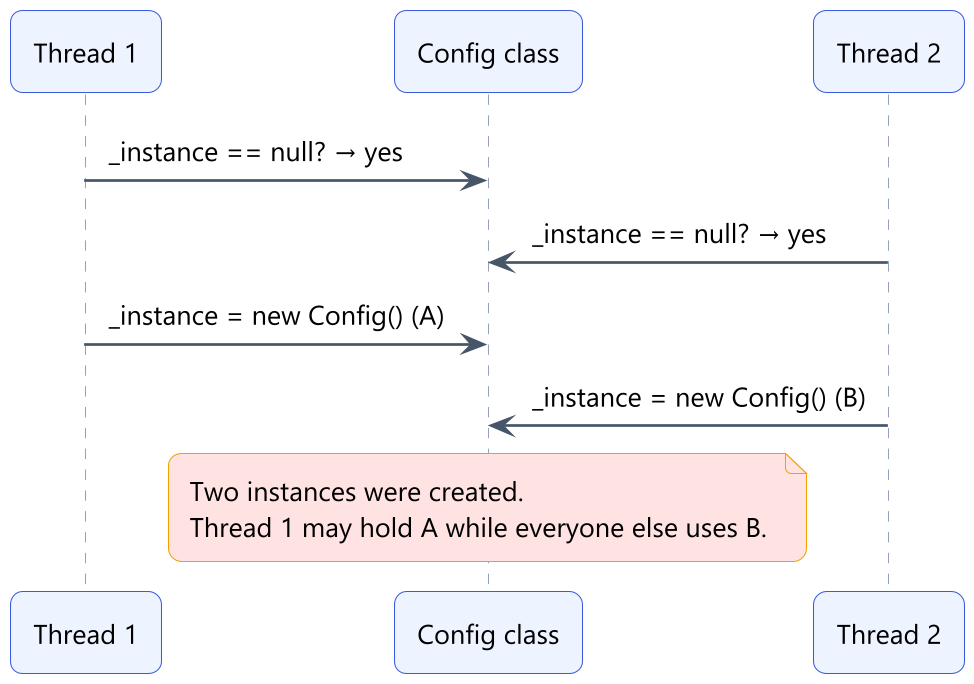
\includegraphics[width=0.92\textwidth,height=0.42\textheight,keepaspectratio]{assets/d14-singleton-race.png}}
\caption{A race in the naive Singleton. Both threads pass the null check before either assigns.}
\end{figure}

\passthrough{\lstinline!Lazy<T>!} removes the race by locking internally during the first creation.

\section{Disadvantages: why Singleton is often criticised}

A Singleton is global state. Any class can call \passthrough{\lstinline!CatalogDefaults.Instance!} without declaring it in its constructor, so its dependencies are hidden, which goes against Dependency Inversion. In a unit test the instance cannot be replaced with a fake, and mutable state in a Singleton leaks from one test to the next. Modern .NET applications usually register a service with a single lifetime in the dependency injection container instead:~\cite{di}

\begin{lstlisting}
services.AddSingleton<ICatalogDefaults, CatalogDefaults>();
\end{lstlisting}

There is still one instance, but classes receive it through their constructors and tests can pass a different one. In Domi the Singleton is limited to immutable defaults. Groups and profiles are per-user data with many instances, so they are never Singletons.

\textbf{Short answer for the defense:} "A Singleton guarantees one object and one global access point. I use it for things that must be shared and the same everywhere, like configuration or a logger; in Domi, the catalog defaults. I don\textquotesingle t use it for user data like groups or profiles, because there are many of them, and I avoid it for anything that changes, because it\textquotesingle s global state that hides dependencies and is hard to test. In modern C\#, the usual way is to register a service as a singleton in dependency injection."

\chapter{Factory Method}

\section{The idea in plain words}

Think of a pizza chain. Every shop follows the same steps: \textbf{make the pizza, bake it, box it}. Only the first step differs: the Italian shop makes thin crust, the American shop thick crust. Head office writes the steps once, and each shop only says how \emph{it} makes the pizza.

In code, the parent class writes the steps, and the "make" step is an \textbf{abstract} method (no body). Each child class \textbf{overrides} that one method, which means it writes its own version of it. That one creating method is the \textbf{factory method}. The other steps are not; they are the fixed workflow around it.

\section{Problem, step by step}

\textbf{Start: creation with \passthrough{\lstinline!if!}.} A service creates groups itself:

\begin{lstlisting}
public Group Create(string type)
{
    if (type == "student") return new Group("Student flat", 300, 5);
    if (type == "quiet")   return new Group("Quiet home", 500, 2);
    throw new Exception("unknown type");
}
\end{lstlisting}

To add "family" groups, you must \textbf{open this method and edit it}. Every edit can break code that already works. This breaks the Open/Closed Principle: add new behavior by adding code, not by editing old code.

\textbf{First fix: Simple Factory.} Move the \passthrough{\lstinline!if!} chain into a separate \passthrough{\lstinline!GroupFactory.Create(type)!}. The service is cleaner, but a new type still means editing the \passthrough{\lstinline!if!} chain. The problem moved; it did not disappear. Simple Factory is a common idiom but not one of the official patterns.

\textbf{Real fix: Factory Method.} Replace the \passthrough{\lstinline!if!} with inheritance. The parent keeps the workflow; each type of group is a child class. A new type is a new class, and no existing code changes.

\section{Where it fits in Domi}

Creating a group with its founder always means: create the group, save the founder\textquotesingle s profile, join them. Only the kind of group differs: a student flat (cheap, five people) or a quiet home (two people).

\section{Code}

\begin{lstlisting}
public abstract class GroupCreator
{
    public GroupView CreateAndJoin(GroupService groups, ProfileService profiles, ProfileInput founder)
    {
        GroupInput draft = CreateGroupDraft();
        GroupView group = groups.CreateGroup(draft);
        ProfileView profile = profiles.CreateProfile(founder);
        return groups.JoinGroup(group.Id, profile.Id);
    }

    protected abstract GroupInput CreateGroupDraft();
}

public sealed class StudentGroupCreator : GroupCreator
{
    protected override GroupInput CreateGroupDraft() => new GroupBuilder()
        .WithName("Student flat")
        .WithMaxMonthlyCost(300)
        .WithCapacity(CatalogDefaults.Instance.DefaultCapacity + 2)
        .Build();
}

public sealed class QuietGroupCreator : GroupCreator
{
    protected override GroupInput CreateGroupDraft() => new GroupBuilder()
        .WithName("Quiet home")
        .WithMaxMonthlyCost(CatalogDefaults.Instance.DefaultMaxMonthlyCost)
        .WithCapacity(2)
        .Build();
}
\end{lstlisting}

\section{How it works}

\passthrough{\lstinline!CreateAndJoin!} is a normal method in the base class and contains the fixed workflow. At its first step it calls \passthrough{\lstinline!CreateGroupDraft()!}, which is \passthrough{\lstinline!abstract!}: the base class does not know what it returns. When the program calls \passthrough{\lstinline!new StudentGroupCreator().CreateAndJoin(...)!}, the runtime dispatches \passthrough{\lstinline!CreateGroupDraft()!} to the \passthrough{\lstinline!StudentGroupCreator!} override. This is \textbf{polymorphism}: the same call in the base class runs different code depending on the actual object.

\passthrough{\lstinline!CreateGroupDraft!} is the \textbf{factory method}. It is \passthrough{\lstinline!protected!} because only the workflow should call it.

\begin{figure}[H]
\centering
\pandocbounded{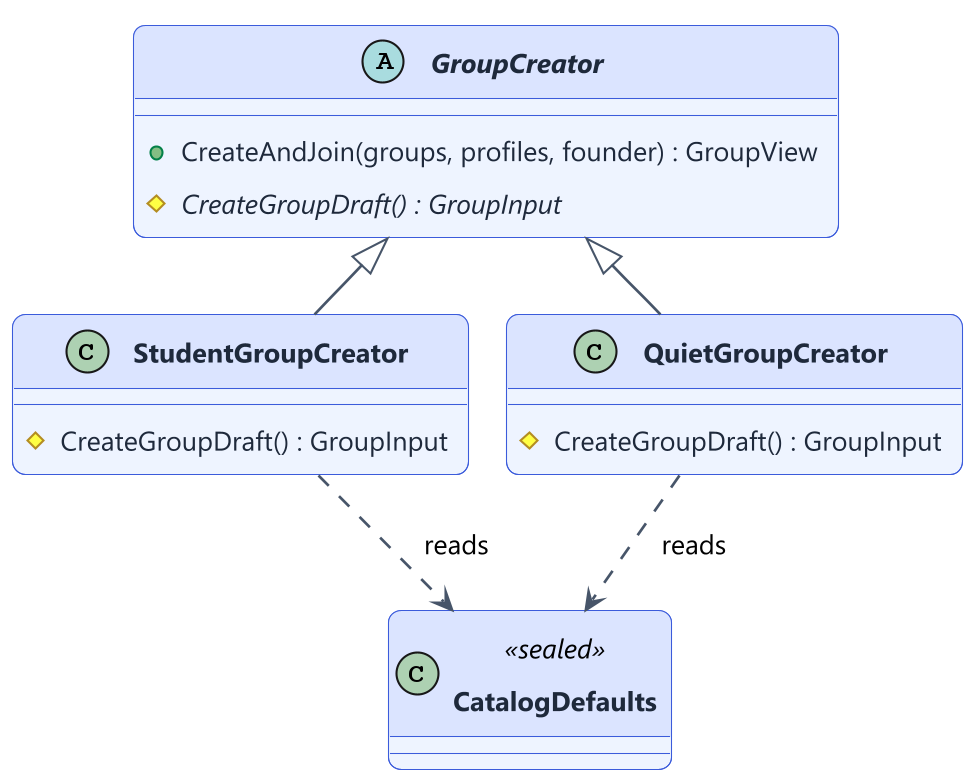
\includegraphics[width=0.92\textwidth,height=0.42\textheight,keepaspectratio]{assets/d15-fm-class.png}}
\caption{Factory Method class diagram. The subclasses override only the creation step.}
\end{figure}

\begin{figure}[H]
\centering
\pandocbounded{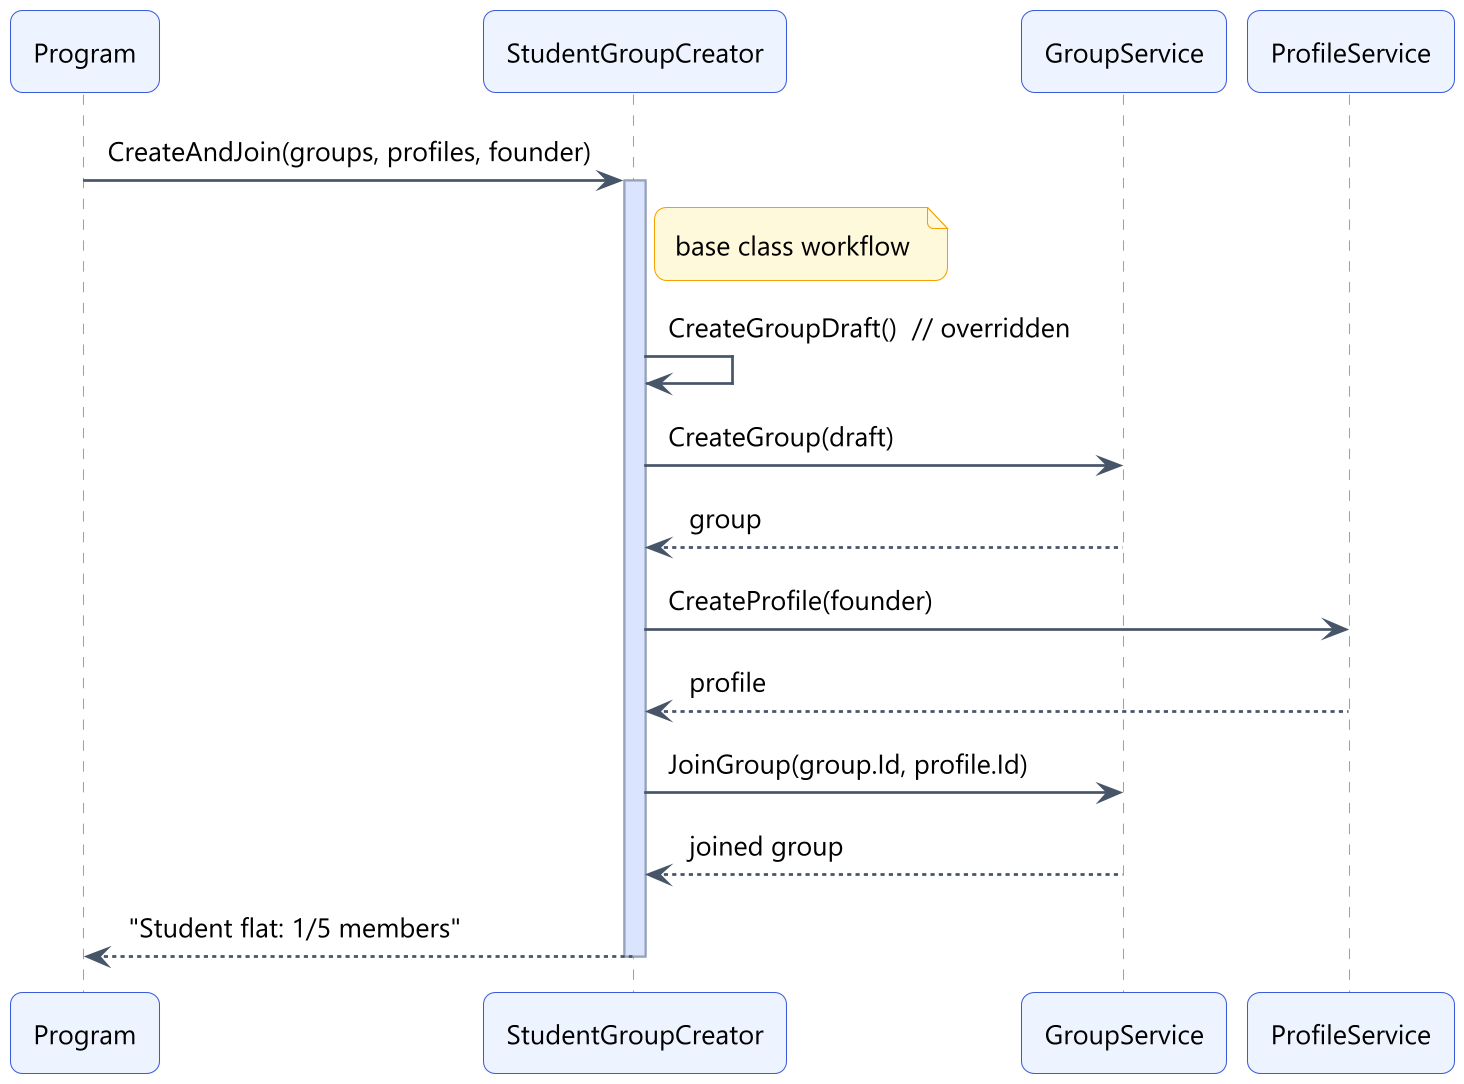
\includegraphics[width=0.92\textwidth,height=0.42\textheight,keepaspectratio]{assets/d16-fm-seq.png}}
\caption{Factory Method sequence. The workflow is inherited; one step is overridden.}
\end{figure}

\section{Factory Method and Abstract Factory compared}

Both create objects through an abstraction, which is why they are easy to confuse. They differ in what they create and in which OOP mechanism varies the result.

{\def\LTcaptype{none} % do not increment counter
\begin{longtable}[]{@{}>{\raggedright\arraybackslash}p{0.320\linewidth}>{\raggedright\arraybackslash}p{0.320\linewidth}>{\raggedright\arraybackslash}p{0.320\linewidth}@{}}
\toprule\noalign{}
& Factory Method & Abstract Factory \\
\midrule\noalign{}
\endhead
\bottomrule\noalign{}
\endlastfoot
Creates & one product & a family of related products \\
Varies through & inheritance: a subclass overrides one method & composition: the client receives a factory object \\
The creating code lives in & a method inside the class that uses the product & a separate factory object \\
In Domi & \passthrough{\lstinline!GroupCreator.CreateGroupDraft()!} & \passthrough{\lstinline!IOnboardingPresetFactory!} \\
\end{longtable}
}

Each method of an Abstract Factory is often implemented as a factory method, so the two patterns frequently appear together.

\textbf{In the analogies:} Factory Method is the pizza chain, where the steps are the same and each shop makes its own crust. Abstract Factory is the furniture style, where one choice gives a whole matching set.

\textbf{Short answer for the defense:} "Factory Method uses inheritance: a child overrides one method to decide which single object is created inside a fixed workflow. Abstract Factory uses an interface: I pass in one factory object that creates a whole family of objects that match each other."

A \textbf{Simple Factory}, a single static method with a \passthrough{\lstinline!switch!} that returns different types, is a common idiom but not one of the Gang of Four patterns. It centralises creation but must be edited for every new type, which Factory Method avoids.

\section{Trade-offs}

Each variant needs a subclass. When variants differ only in data, a parameter or a Builder is simpler than a class hierarchy.

\chapter{Object Pool}

\section{The idea in plain words}

Think of a library. Instead of buying a new book every time someone wants to read, the library keeps its books. You \textbf{borrow} one, read it, and \textbf{return} it, and the next person borrows the same book.

An Object Pool keeps finished objects on a shelf. Code \textbf{acquires} (borrows) one, uses it, and \textbf{releases} (returns) it. If the shelf is empty, the pool creates a new object.

\section{Problem}

Some objects are expensive to create or exist in limited numbers: database connections, threads, network sockets, large buffers. Opening a database connection means reaching the server over the network and logging in, which takes far longer than running a query. A database also accepts only a fixed number of connections at once. Creating and destroying a connection for every request is slow and can hit that limit.

\section{Where it fits in Domi}

Domi builds short text summaries of groups. The pool reuses \passthrough{\lstinline!StringBuilder!} buffers between summaries. In a production backend the same idea is applied to database connections; ADO.NET keeps a connection pool for each connection string, and \passthrough{\lstinline!ArrayPool<T>.Shared!} does the same for arrays~\cite{arraypool}.

\section{Code}

\begin{lstlisting}
public sealed class SummaryBuilderPool(int maxIdle)
{
    private readonly Stack<StringBuilder> _idle = new();

    public int Created { get; private set; }

    public StringBuilder Acquire()
    {
        if (_idle.Count > 0) return _idle.Pop();
        Created++;
        return new StringBuilder();
    }

    public void Release(StringBuilder builder)
    {
        builder.Clear();
        if (_idle.Count < maxIdle) _idle.Push(builder);
    }

    public string Summarize(GroupView group)
    {
        StringBuilder sb = Acquire();
        try
        {
            return sb.Append(group.Name).Append(": ")
                .Append(group.MemberCount).Append('/').Append(group.Capacity)
                .Append(" members, ").Append(group.MaxMonthlyCost).Append(" per month")
                .ToString();
        }
        finally
        {
            Release(sb);
        }
    }
}
\end{lstlisting}

\section{How it works}

The pool keeps idle objects on a stack.

\begin{itemize}
\tightlist
\item \textbf{Acquire} returns an idle builder if there is one. Otherwise it creates a new one and counts it in \passthrough{\lstinline!Created!};
\item \textbf{Release} clears the builder and puts it back, unless the pool already holds \passthrough{\lstinline!maxIdle!} idle builders. In that case the builder is dropped and the garbage collector frees it;
\item \textbf{Summarize} shows the correct usage: acquire, use, and release in \passthrough{\lstinline!finally!}, so the builder returns to the pool even when an exception is thrown;
\end{itemize}

The demo creates two summaries with one pool and prints \passthrough{\lstinline!Pool created 1 StringBuilder(s) for 2 summaries!}: the second summary reused the first builder.

\begin{figure}[H]
\centering
\pandocbounded{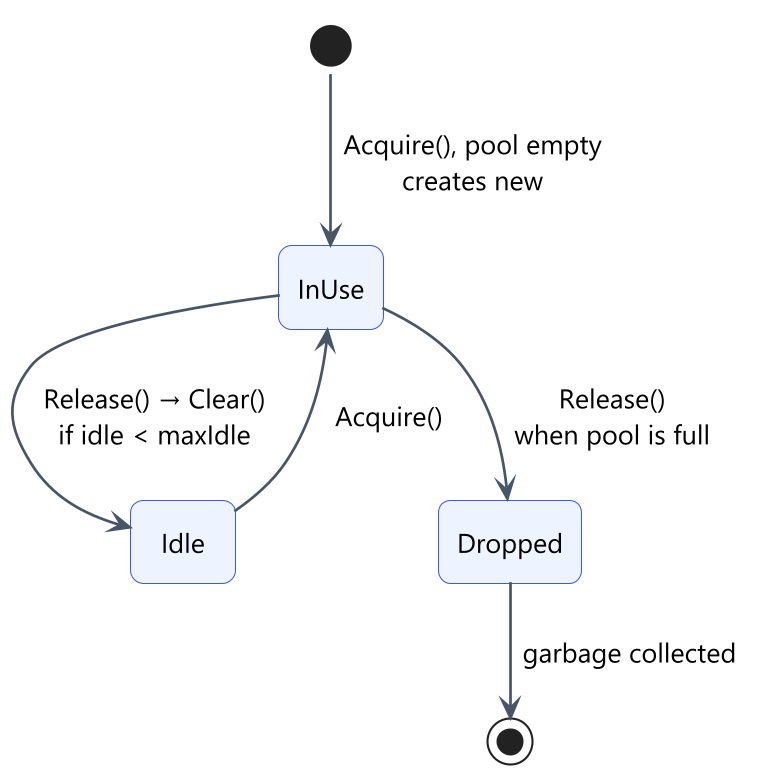
\includegraphics[width=0.92\textwidth,height=0.42\textheight,keepaspectratio]{assets/d17-pool-state.png}}
\caption{Life cycle of a pooled object.}
\end{figure}

\begin{figure}[H]
\centering
\pandocbounded{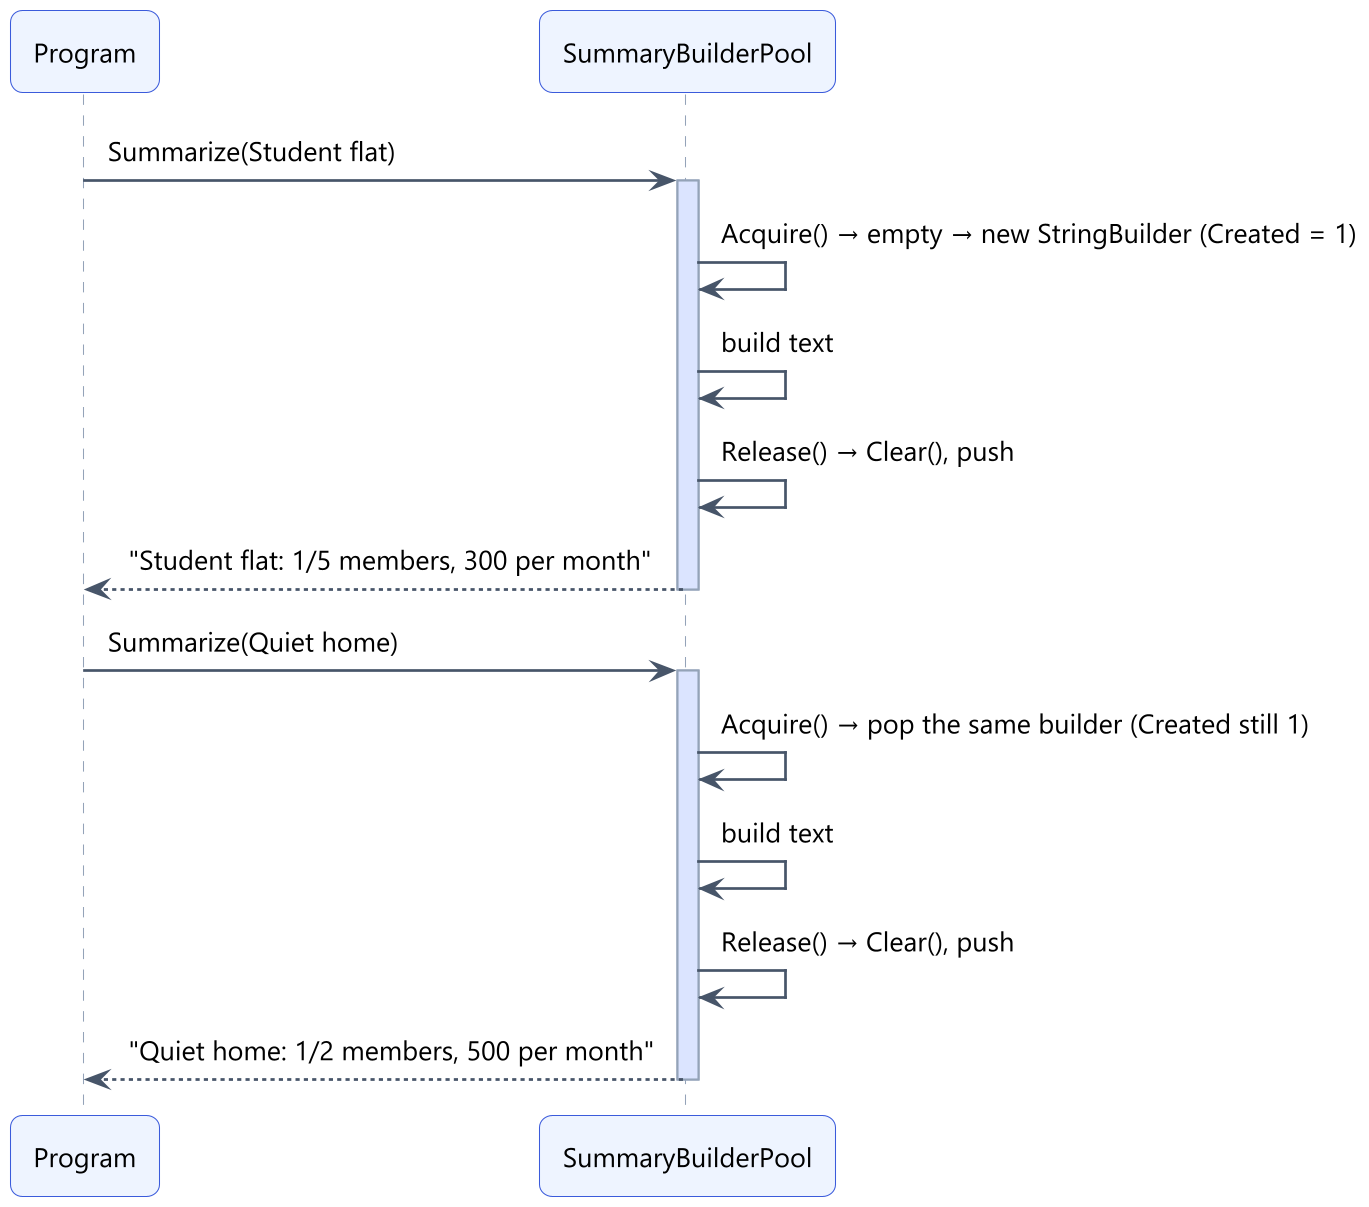
\includegraphics[width=0.92\textwidth,height=0.42\textheight,keepaspectratio]{assets/d18-pool-seq.png}}
\caption{Two summaries, one builder.}
\end{figure}

\begin{figure}[H]
\centering
\pandocbounded{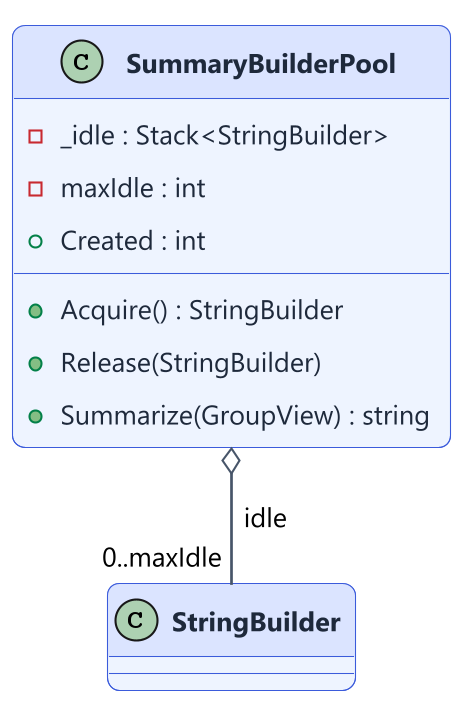
\includegraphics[width=0.92\textwidth,height=0.42\textheight,keepaspectratio]{assets/d19-pool-class.png}}
\caption{Object Pool class diagram.}
\end{figure}

\section{The two rules of pooling}

\begin{enumerate}
\def\labelenumi{\arabic{enumi}.}
\tightlist
\item \textbf{Reset on release.} Without \passthrough{\lstinline!Clear()!}, the next user would receive a builder that still contains the previous summary. With database connections the same mistake leaks an open transaction or another user\textquotesingle s session settings;
\item \textbf{Always release.} If a user acquires an object and an exception skips the release, the object never returns, like a library book that is never brought back. A pool without a limit keeps creating new objects and the benefit is lost. A pool with a hard limit, such as 100 database connections, is worse: after 100 lost connections, the 101st request \textbf{waits forever} and the application hangs. \passthrough{\lstinline!try/finally!} (or \passthrough{\lstinline!using!} with a disposable wrapper) prevents this, because \passthrough{\lstinline!finally!} runs even after an error;
\end{enumerate}

\passthrough{\lstinline!maxIdle!} caps how much the pool holds when demand drops, so a burst of traffic does not leave memory reserved forever.

\section{Trade-offs}

Pooling pays off only when creation is expensive compared with the bookkeeping. A small \passthrough{\lstinline!StringBuilder!} is cheap, and the .NET garbage collector handles short-lived objects efficiently, so in Domi the pool is mainly a clear demonstration of the mechanism. This pool is also not thread-safe; a shared pool used by several threads would need \passthrough{\lstinline!ConcurrentBag<T>!} or a lock.

\chapter{How the patterns work together}

\begin{figure}[H]
\centering
\pandocbounded{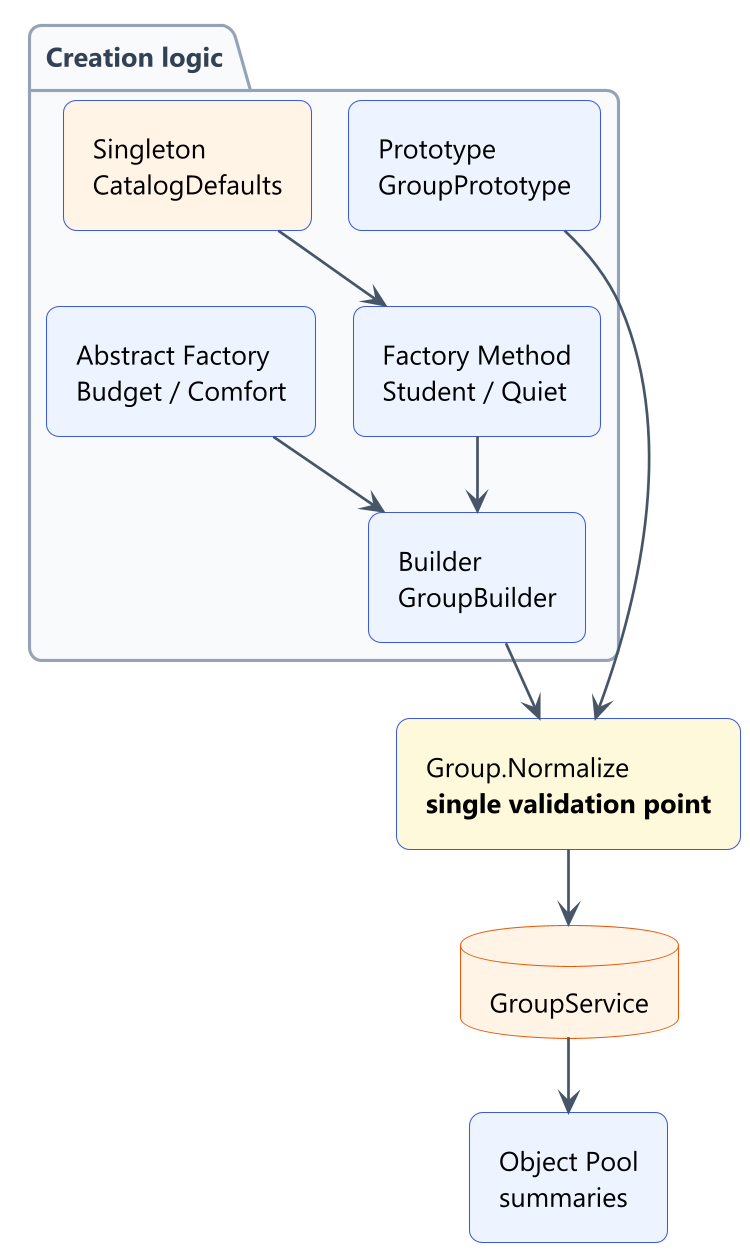
\includegraphics[width=0.92\textwidth,height=0.42\textheight,keepaspectratio]{assets/d20-together.png}}
\caption{Every creation path ends in \protect\passthrough{\lstinline!Group.Normalize!} before the service stores the group.}
\end{figure}

The patterns combine instead of competing. Both factories use the Builder to assemble their group drafts, the Factory Method creators read defaults from the Singleton, and the Prototype goes through the same constructor as everything else. Because every path converges on one validation method, adding a new creation path cannot weaken the rules.

\section{Connection to SOLID (Lab 0)}

{\def\LTcaptype{none} % do not increment counter
\begin{longtable}[]{@{}>{\raggedright\arraybackslash}p{0.480\linewidth}>{\raggedright\arraybackslash}p{0.480\linewidth}@{}}
\toprule\noalign{}
Principle & Where this lab applies it \\
\midrule\noalign{}
\endhead
\bottomrule\noalign{}
\endlastfoot
Single Responsibility & The Builder assembles, \passthrough{\lstinline!Normalize!} validates, the services store. The Prototype only copies. \\
Open/Closed & A new onboarding family or a new group creator is a new class; existing code does not change. \\
Liskov Substitution & Any \passthrough{\lstinline!IOnboardingPresetFactory!} or \passthrough{\lstinline!GroupCreator!} subclass can replace another without breaking the caller. \\
Interface Segregation & \passthrough{\lstinline!IOnboardingPresetFactory!} contains only the two methods onboarding needs. \\
Dependency Inversion & \passthrough{\lstinline!Presets.Build!} depends on \passthrough{\lstinline!IOnboardingPresetFactory!}, not on concrete factories. The Singleton section explains where it conflicts with this principle and how DI fixes it. \\
\end{longtable}
}

\section{Choosing a pattern}

\begin{figure}[H]
\centering
\pandocbounded{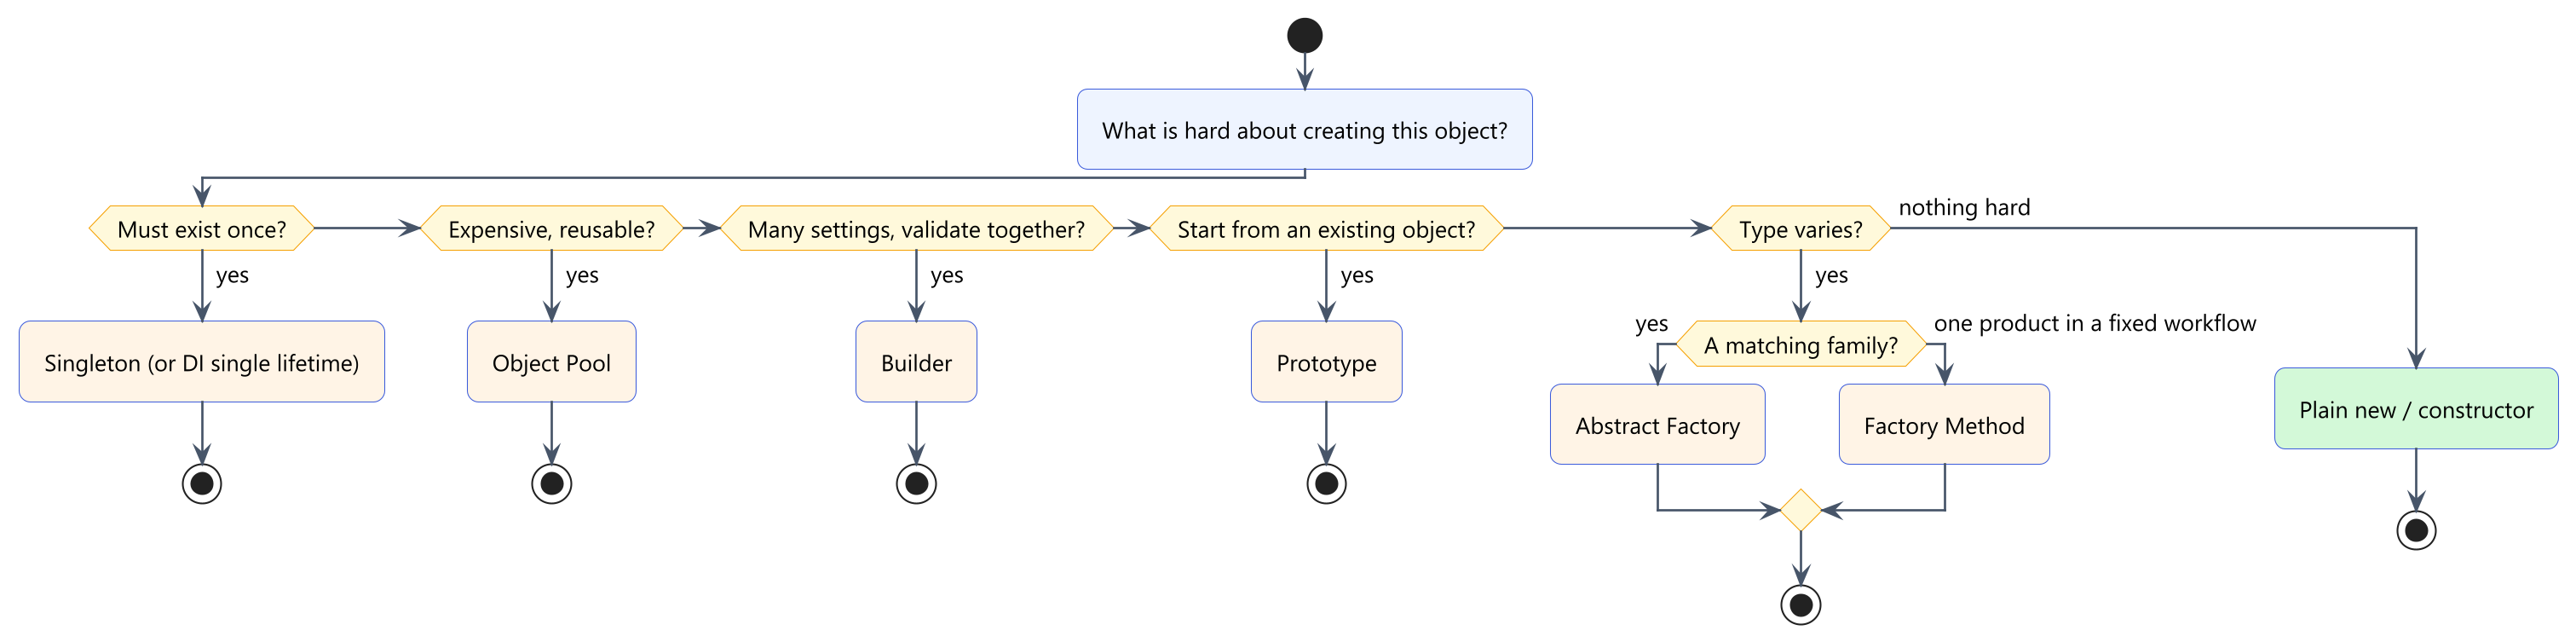
\includegraphics[width=0.92\textwidth,height=0.42\textheight,keepaspectratio]{assets/d21-decision.png}}
\caption{A decision guide. "Nothing hard" is a valid answer: patterns are for problems that exist.}
\end{figure}

\chapter{Results}

Running \passthrough{\lstinline!dotnet run!}:

\begin{lstlisting}
{
  "builderGroup": { "id": "group-1", "name": "Builder example home", "maxMonthlyCost": 650, "capacity": 3, "memberCount": 0 },
  "presetGroups": [
    {
      "family": "budget",
      "group": { "id": "group-2", "name": "Budget shared home", "maxMonthlyCost": 450, "capacity": 4, "memberCount": 1 },
      "suggestedProfile": { "id": "profile-1", "name": "Budget renter" }
    },
    {
      "family": "comfort",
      "group": { "id": "group-3", "name": "Comfort shared home", "maxMonthlyCost": 700, "capacity": 2, "memberCount": 1 },
      "suggestedProfile": { "id": "profile-2", "name": "Comfort renter" }
    }
  ],
  "prototype": {
    "sourceGroupId": "group-2",
    "sourceMemberCount": 1,
    "copy": { "id": "group-4", "name": "Budget shared home copy", "maxMonthlyCost": 450, "capacity": 4, "memberCount": 0 }
  }
}
\end{lstlisting}

{\def\LTcaptype{none} % do not increment counter
\begin{longtable}[]{@{}>{\raggedright\arraybackslash}p{0.480\linewidth}>{\raggedright\arraybackslash}p{0.480\linewidth}@{}}
\toprule\noalign{}
Output & What it shows \\
\midrule\noalign{}
\endhead
\bottomrule\noalign{}
\endlastfoot
\passthrough{\lstinline!builderGroup!} is \passthrough{\lstinline!group-1!} with the three values set & The Builder produced a valid input that the service saved. \\
Both preset groups have \passthrough{\lstinline!memberCount: 1!} & Each factory produced a matching pair, so the suggested renter could join. \\
The prototype source has 1 member, the copy has 0 and a new ID \passthrough{\lstinline!group-4!} & The clone copied the settings, not the identity or the members, and the source was not affected. \\
\end{longtable}
}

Running \passthrough{\lstinline!dotnet run -- --extra!}:

\begin{lstlisting}
Singleton same instance: True
Student flat: 1/5 members, 300 per month
Quiet home: 1/2 members, 500 per month
Pool created 1 StringBuilder(s) for 2 summaries
\end{lstlisting}

{\def\LTcaptype{none} % do not increment counter
\begin{longtable}[]{@{}>{\raggedright\arraybackslash}p{0.480\linewidth}>{\raggedright\arraybackslash}p{0.480\linewidth}@{}}
\toprule\noalign{}
Output & What it shows \\
\midrule\noalign{}
\endhead
\bottomrule\noalign{}
\endlastfoot
\passthrough{\lstinline!same instance: True!} & Two reads of \passthrough{\lstinline!CatalogDefaults.Instance!} return the same object. \\
Student 1/5 at 300, Quiet 1/2 at 500 & One inherited workflow, two different overridden creation steps. Capacity 5 and cost 500 come from the Singleton\textquotesingle s defaults. \\
\passthrough{\lstinline!Created 1 ... for 2 summaries!} & The second summary reused the pooled builder. \\
\end{longtable}
}

\section{Project structure}

\begin{lstlisting}
lab-01/csharp/
  DomiLab01.csproj   .NET 8 console project
  Domain.cs          Group, Profile, inputs, views, validation
  Services.cs        GroupService, ProfileService
  Patterns.cs        Builder, Abstract Factory, Prototype
  ExtraPatterns.cs   Singleton, Factory Method, Object Pool
  Program.cs         Demo for both runs
\end{lstlisting}

\utmconclusions
Creating an object becomes a design problem when the caller should not depend on the concrete class, when construction has rules that must hold together, or when the number of instances matters. This lab applied the six creational patterns to those situations in Domi.

The \textbf{Builder} made group creation readable and validated it once at the end. The \textbf{Abstract Factory} guaranteed that an onboarding group and its suggested renter always match, and showed its trade-off: new families are cheap, new product types are not. The \textbf{Prototype} reused a group\textquotesingle s settings while deliberately leaving out its identity and members, which made the difference between a shallow and a deep copy concrete. The \textbf{Singleton} gave one shared set of defaults, together with the reasons it is usually replaced by a dependency injection lifetime. The \textbf{Factory Method} kept one workflow and let subclasses choose the group, which is the inheritance-based counterpart to Abstract Factory. The \textbf{Object Pool} reused buffers and showed the two rules that make pooling safe: reset on release and always release.

The most useful lesson is that the patterns serve the SOLID principles from Lab 0. They move the decision of \emph{what to create} away from the code that \emph{uses} the object, so that new kinds of groups, families and copies can be added without editing the code that already works.


\begin{thebibliography}{9}
\bibitem{gof} E. Gamma, R. Helm, R. Johnson, J. Vlissides. \textit{Design Patterns: Elements of Reusable Object-Oriented Software}. Addison-Wesley, 1994.
\bibitem{lazy} Microsoft. \textit{Lazy<T> Class}. Available online: \url{https://learn.microsoft.com/dotnet/api/system.lazy-1} (accessed on 3 November 2026).
\bibitem{di} Microsoft. \textit{Dependency injection in .NET: service lifetimes}. Available online: \url{https://learn.microsoft.com/dotnet/core/extensions/dependency-injection} (accessed on 3 November 2026).
\bibitem{arraypool} Microsoft. \textit{ArrayPool<T> Class}. Available online: \url{https://learn.microsoft.com/dotnet/api/system.buffers.arraypool-1} (accessed on 3 November 2026).
\end{thebibliography}
\end{document}
